\documentclass[twoside,spanish,a4paper,12pt]{tfg}

\usepackage{booktabs}
\usepackage{tabularx}
\usepackage{array}
\usepackage{float}
\usepackage{booktabs}
\usepackage{tabularx}
\usepackage{array}
\usepackage{float}
\usepackage{amsmath}
\usepackage{xcolor}
\usepackage{colortbl}
\usepackage{booktabs}
\usepackage{tabularx}
\usepackage{array}
\usepackage{float}
\usepackage{amsmath}

% Evita que LaTeX estire verticalmente las páginas con muchas figuras [H]
% (el espacio sobrante queda al final de la página en vez de repartirse entre
% párrafos), eliminando el espaciado vertical irregular del capítulo de resultados.
\raggedbottom

% Editar la titulación
\titulacion{Grado en Ciencia de Datos}

% Editar el título
\title{Diagnóstico de lesiones de rodilla utilizando imágenes de resonancia magnética}

% Si es una alumna se debe usar
% \authorlabel{Autora}
\authorlabel{Autor}
% Editar el nombre
\author{Pablo López Domínguez}


% Si hay varios tutores:
\tutorlabel{Tutores}
\tutor{\shortstack[l]{\\[2mm] José David Martín Guerrero \\[4pt] Yolanda Vives Gilabert}}
% Si el tutor es masculino:
% \tutorlabel{Tutor}
%\tutorlabel{Tutora}
% Editar
%\tutor{El nombre de la tutora}

% Editar: Poner mes y año de la convocatoria de lectura del TFM
\convocatoria{Julio 2026}

% Renombrar "Cuadro" -> "Tabla" en captions e índice
\addto\captionsspanish{%
  \renewcommand{\tablename}{Tabla}%
  \renewcommand{\listtablename}{Índice de tablas}%
}

\begin{document}

% NO QUITAR ESTOS ELEMENTOS
\portada
\cleardoublepage
\contraportada
\cleardoublepage
\declaracion
\cleardoublepage


% Editar: Resumen en Español
\begin{resumen}
El diagnóstico de lesiones de rodilla mediante imágenes de resonancia magnética (RM) constituye un proceso fundamental en la práctica clínica, que exige un elevado grado de especialización y un considerable consumo de tiempo por parte de los profesionales sanitarios. En este contexto, el presente trabajo aborda la aplicación de técnicas avanzadas de aprendizaje profundo con el objetivo de automatizar y optimizar la detección de patologías en imágenes médicas.

Concretamente, se han implementado y evaluado tres arquitecturas representativas del estado del arte en visión por computador: una red neuronal convolucional profunda (ResNet) y dos modelos basados en mecanismos de atención tipo transformer (Vision Transformer y Swin Transformer). Dichos modelos han sido entrenados y validados sobre un conjunto de datos de imágenes de resonancia magnética de rodilla, con el propósito de analizar su capacidad para identificar patrones relevantes asociados a distintos tipos de lesiones.

Los resultados obtenidos permiten establecer una comparación rigurosa entre los diferentes enfoques, poniendo de manifiesto las ventajas y limitaciones de cada arquitectura en términos de precisión, capacidad de generalización y eficiencia computacional. Asimismo, se discuten las implicaciones de estos hallazgos en el ámbito clínico, así como las principales limitaciones del estudio.

Finalmente, se proponen diversas líneas de investigación futura orientadas a mejorar la robustez y la aplicabilidad de estos modelos en entornos clínicos reales. Este trabajo contribuye al avance del uso de técnicas de aprendizaje profundo en el diagnóstico médico, evidenciando el potencial de las arquitecturas basadas en transformers frente a enfoques tradicionales basados en convoluciones.
\end{resumen}
\cleardoublepage

% Editar: Resumen en Inglés
\begin{abstract}
The diagnosis of knee injuries using magnetic resonance imaging (MRI) is a fundamental task in clinical practice, requiring a high level of expertise and a significant investment of time from medical professionals. In this context, this work explores the application of advanced deep learning techniques with the aim of automating and enhancing the detection of pathologies in medical images.

Specifically, three representative state-of-the-art computer vision architectures have been implemented and evaluated: a deep convolutional neural network (ResNet) and two transformer-based models (Vision Transformer and Swin Transformer). These models have been trained and validated on a dataset of knee MRI images in order to assess their ability to identify relevant patterns associated with different types of injuries.

The obtained results enable a rigorous comparison between the different approaches, highlighting the strengths and limitations of each architecture in terms of accuracy, generalization capability, and computational efficiency. Furthermore, the implications of these findings in the clinical domain are discussed, along with the main limitations of the study.

Finally, several future research directions are proposed to improve the robustness and applicability of these models in real clinical environments. This work contributes to the advancement of deep learning techniques in medical diagnosis, demonstrating the potential of transformer-based architectures compared to traditional convolutional approaches.
\end{abstract}
\cleardoublepage

% Editar: Resumen en Valenciano
\begin{resumen}
El diagnòstic de lesions de genoll mitjançant imatges de ressonància magnètica (RM) constitueix una tasca fonamental en la pràctica clínica, que requereix un alt nivell d’especialització i un considerable consum de temps per part dels professionals sanitaris. En aquest context, el present treball aborda l’aplicació de tècniques avançades d’aprenentatge profund amb l’objectiu d’automatitzar i millorar la detecció de patologies en imatges mèdiques.

Concretament, s’han implementat i avaluat tres arquitectures representatives de l’estat de l’art en visió per computador: una xarxa neuronal convolucional profunda (ResNet) i dos models basats en mecanismes d’atenció de tipus transformer (Vision Transformer i Swin Transformer). Aquests models han sigut entrenats i validats sobre un conjunt de dades d’imatges de ressonància magnètica de genoll, amb la finalitat d’analitzar la seua capacitat per identificar patrons rellevants associats a diferents tipus de lesions.

Els resultats obtinguts permeten establir una comparació rigorosa entre els diferents enfocaments, posant de manifest les fortaleses i limitacions de cada arquitectura en termes de precisió, capacitat de generalització i eficiència computacional. Així mateix, es discuteixen les implicacions d’aquests resultats en l’àmbit clínic, així com les principals limitacions de l’estudi.

Finalment, es proposen diverses línies de treball futur orientades a millorar la robustesa i l’aplicabilitat d’aquests models en entorns clínics reals. Aquest treball contribueix a l’avanç de les tècniques d’aprenentatge profund en el diagnòstic mèdic, evidenciant el potencial de les arquitectures basades en transformers enfront dels enfocaments tradicionals basats en convolucions.
\end{resumen}
\cleardoublepage



% Editar: Agradecimientos (opcional)
\begin{agradecimientos}

En primer lugar, quiero expresar mi más sincero agradecimiento a mis tutores, David y Yolanda, por su orientación, apoyo y dedicación a lo largo de la realización de este trabajo. Su experiencia, sus consejos y su disponibilidad han sido fundamentales para el desarrollo de este proyecto.

\vspace{0.5em}

Asimismo, me gustaría agradecer a todos los profesores que han formado parte de mi formación académica durante estos años, por haber contribuido a mi aprendizaje y haber despertado mi interés por el ámbito de la Ciencia de Datos.

\vspace{0.5em}

De manera especial, quiero dar las gracias a mis amigos y compañeros, por su apoyo constante, motivación y por compartir conmigo este camino.

\vspace{0.5em}

Quiero también agradecer especialmente a Laura, por haberme apoyado de manera incondicional durante toda la carrera, por su paciencia, su comprensión y por haber estado a mi lado incluso en los momentos más difíciles. Este camino habría sido mucho más difícil sin ti.

\vspace{0.5em}

Finalmente, quiero expresar mi más profundo agradecimiento a mi familia y seres queridos, por su apoyo incondicional, su paciencia y su confianza en mí a lo largo de toda esta etapa. Sin ellos, nada de esto habría sido posible.

\end{agradecimientos}
\cleardoublepage

\tableofcontents

\pagestyle{tfg}
\justify

% Las figuras se buscan en el directorio figs

% Cada capítulo está en su propio fichero tex. Ver el directorio tex.

% La bibliografía está dentro del directorio bib
\chapter{Introducción}
% Contenidos del capítulo.
% Las secciones presentadas son orientativas y no representan
% necesariamente la organización que debe tener este capítulo.


\section{Contexto y Motivación}

El diagnóstico de lesiones de rodilla constituye un desafío relevante en el ámbito de la medicina deportiva, especialmente en contextos de alta exigencia física donde la incidencia de patologías articulares, como la rotura del ligamento cruzado anterior (ACL), es especialmente elevada. Este tipo de lesiones no solo tiene un impacto inmediato en el rendimiento deportivo, sino que también puede condicionar la trayectoria profesional de los deportistas y afectar a su calidad de vida a largo plazo.

En estos escenarios, la resonancia magnética (RM) se erige como una herramienta fundamental para la evaluación clínica, permitiendo la identificación precisa de lesiones en estructuras internas de la articulación como ligamentos, meniscos o cartílago. Su carácter no invasivo y su alta capacidad de resolución la convierten en una técnica indispensable dentro del proceso diagnóstico. No obstante, la interpretación de estas imágenes requiere un alto grado de especialización y experiencia por parte de los radiólogos.

En la práctica clínica, este proceso de análisis suele estar condicionado por la elevada carga asistencial, lo que puede traducirse en tiempos de espera significativos para la obtención de un informe diagnóstico. Esta situación resulta especialmente crítica en contextos deportivos, donde la rapidez en la toma de decisiones puede influir directamente en el tratamiento, la recuperación y la planificación del retorno a la actividad.

La motivación de este trabajo surge tanto del interés académico como de la experiencia personal en el ámbito del deporte de alto nivel durante la etapa de formación, compitiendo en entornos de elevada exigencia. Este tipo de contextos, caracterizados por una gran intensidad competitiva y física, implican también una mayor exposición a lesiones de gravedad.

En este sentido, he sufrido varias lesiones de rodilla de carácter severo, incluyendo roturas del ligamento cruzado anterior, que han requerido múltiples intervenciones quirúrgicas y un seguimiento clínico prolongado basado en la realización de numerosas resonancias magnéticas. A lo largo de este proceso, he podido observar de manera directa no solo la importancia crítica del diagnóstico por imagen, sino también las limitaciones existentes en términos de tiempo de respuesta, acceso a especialistas y necesidad de interpretación experta.

Esta experiencia despertó un interés inicial por comprender e interpretar las imágenes de resonancia magnética de rodilla, motivado tanto por la necesidad personal como por la curiosidad técnica. Paralelamente, durante el desarrollo del Grado en Ciencia de Datos, los conocimientos adquiridos en áreas como el aprendizaje automático, el análisis de datos y la visión por computador permitieron identificar el potencial de estas tecnologías para abordar problemas complejos en el ámbito médico.

En los últimos años, el avance de las técnicas de aprendizaje profundo ha supuesto un cambio significativo en el campo de la visión por computador, permitiendo desarrollar modelos capaces de extraer patrones complejos a partir de grandes volúmenes de datos. Estas capacidades abren la puerta a su aplicación en el análisis de imágenes médicas, donde pueden actuar como herramientas de apoyo en la detección de patologías.

A partir de esta combinación de experiencia personal y formación académica, surge la idea de explorar el uso de herramientas basadas en aprendizaje profundo para asistir en la detección de lesiones a partir de imágenes médicas. De este modo, este proyecto se sitúa en la intersección entre una problemática clínica real y las capacidades tecnológicas actuales, con la finalidad de analizar posibles soluciones que contribuyan a mejorar la eficiencia del proceso diagnóstico y el apoyo a los profesionales sanitarios.


\section{Objetivos}

El objetivo principal de este trabajo es analizar el potencial de técnicas de aprendizaje profundo en la detección de lesiones de rodilla a partir de imágenes de resonancia magnética, evaluando su aplicabilidad como herramientas de apoyo en el ámbito clínico.

Para alcanzar este objetivo general, se plantean los siguientes objetivos específicos:

\begin{itemize}
    \item Estudiar el estado del arte en el uso de técnicas de visión por computador y aprendizaje profundo aplicadas al análisis de imágenes médicas, con especial atención al diagnóstico de lesiones de rodilla.
    
    \item Seleccionar, implementar y adaptar distintas arquitecturas representativas del estado del arte, incluyendo modelos basados en redes neuronales convolucionales (ResNet) y modelos basados en transformers (Vision Transformer y Swin Transformer).
    
    \item Preparar y procesar un conjunto de datos de imágenes de resonancia magnética de rodilla, incluyendo tareas de preprocesado, normalización y partición en conjuntos de entrenamiento, validación y prueba.
    
    \item Entrenar los modelos seleccionados y ajustar sus parámetros con el fin de optimizar su rendimiento en la tarea de clasificación o detección de lesiones.
    
    \item Evaluar de forma rigurosa el rendimiento de los diferentes modelos mediante métricas adecuadas, analizando su precisión, capacidad de generalización y eficiencia computacional.
    
    \item Comparar los resultados obtenidos entre las distintas arquitecturas, identificando sus principales fortalezas y limitaciones en el contexto del problema abordado.
    
    \item Analizar la viabilidad del uso de estos modelos como herramientas de apoyo al diagnóstico clínico, considerando tanto sus ventajas como sus posibles limitaciones en entornos reales.
  
\end{itemize}


\section{Estado del Arte}

En los últimos años, el uso de técnicas de aprendizaje profundo en imagen médica ha experimentado un crecimiento notable, especialmente en tareas de clasificación, detección y segmentación sobre imágenes de resonancia magnética (RM). En el caso concreto del diagnóstico de lesiones de rodilla, este avance ha estado impulsado por la disponibilidad de conjuntos de datos públicos y por la mejora progresiva de las arquitecturas de visión por computador. En este contexto, la detección automatizada de lesiones del ligamento cruzado anterior (LCA) a partir de imágenes de resonancia magnética se ha consolidado como una línea de investigación de gran relevancia.

A nivel metodológico, una parte importante de la investigación reciente se ha centrado en el desarrollo de modelos de clasificación directa de extremo a extremo (\textit{end-to-end}). Aunque existen propuestas que plantean sistemas híbridos basados en una segmentación o localización previa de la región de interés antes de realizar la clasificación, este Trabajo de Fin de Grado se enmarca dentro de los enfoques de clasificación directa. Esta decisión responde a criterios de aplicabilidad práctica y viabilidad clínica, fundamentados en tres razones principales:

\begin{itemize}
    \item \textbf{Coste de anotación:} Los modelos de segmentación requieren máscaras detalladas a nivel de píxel o vóxel, delineadas manualmente por radiólogos expertos en cada uno de los cortes bidimensionales del volumen. Este proceso supone un recurso limitado y costoso en el ámbito médico.
    \item \textbf{Propagación del error:} En sistemas en cascada, formados por una etapa de segmentación seguida de una etapa de clasificación, cualquier imprecisión cometida al delimitar el ligamento puede trasladarse al clasificador y afectar al diagnóstico final.
    \item \textbf{Preservación de signos indirectos de lesión:} En la práctica clínica, el estado del ligamento no se evalúa de forma aislada, sino junto con indicios periféricos relevantes, como el edema óseo por contusión (\textit{bone bruising}) en el cóndilo femoral lateral o la traslación tibial anterior. Un clasificador directo procesa el volumen completo de la articulación, permitiendo al modelo aprender estas relaciones contextuales.
\end{itemize}

Por todo ello, la comparación sistemática entre arquitecturas convolucionales y modelos basados en mecanismos de atención aplicados a la clasificación directa constituye uno de los ejes principales del debate científico actual y del presente trabajo.

\subsection{El conjunto de datos MRNet como referencia}

Uno de los principales hitos en este ámbito es la publicación del conjunto de datos \textit{MRNet}, desarrollado por el \textit{Stanford Machine Learning Group} en 2018 \cite{bien2018deep}, que se ha convertido en una referencia habitual para la evaluación de modelos de aprendizaje profundo aplicados al análisis de resonancias magnéticas de rodilla. Este dataset está compuesto por 1.370 estudios de RM de rodilla e incluye etiquetas para tres tareas diagnósticas: anormalidad general, lesión meniscal y rotura del ligamento cruzado anterior.

Para el estudio del LCA, la serie sagital ponderada en T2 con supresión grasa resulta especialmente relevante, ya que permite visualizar con claridad la continuidad de las fibras del ligamento. No obstante, uno de los aspectos más importantes al revisar la literatura es que los protocolos de evaluación no siempre son homogéneos, lo que dificulta la comparación directa entre trabajos.

En particular, conviene distinguir entre la nomenclatura empleada en el artículo original y la utilizada en el contexto competitivo asociado a MRNet. En muchos trabajos posteriores, el conjunto de validación pública se utiliza como referencia principal, mientras que el denominado \textit{hidden test set} permanece oculto y solo puede evaluarse mediante la plataforma de competición de Stanford. Como consecuencia, gran parte de los resultados reportados en la literatura corresponden a validación pública o a particiones propias definidas por los autores, y no al conjunto de test oculto.

\begin{table}[H]
\centering
\small
\caption{Correspondencia entre las particiones de MRNet y su uso en el artículo original y en la competición.}
\label{tab:mrnet_splits}
\begin{tabularx}{\textwidth}{
>{\raggedright\arraybackslash}X
>{\centering\arraybackslash}m{2.1cm}
>{\centering\arraybackslash}m{3cm}
>{\centering\arraybackslash}m{3.4cm}
}
\toprule
\textbf{Segmento} &
\textbf{N.\textsuperscript{o} de estudios} &
\textbf{Artículo original} &
\textbf{Uso habitual posterior} \\
\midrule
Entrenamiento &
1130 &
\textit{Training set} &
\textit{Training set} \\

Validación pública &
120 &
\textit{Tuning set} &
\textit{Validation set} \\

Test oculto &
120 &
\textit{Validation set} &
\textit{Hidden test set} \\
\bottomrule
\end{tabularx}
\end{table}

Esta distinción es especialmente importante desde el punto de vista metodológico, ya que un resultado obtenido sobre validación pública no debe interpretarse como directamente comparable con otro obtenido sobre el test oculto. En consecuencia, cualquier revisión del estado del arte debe considerar no solo la métrica reportada, sino también el protocolo exacto de evaluación empleado.

\subsection{Primeros enfoques basados en redes convolucionales (ResNet)}

El trabajo original de \textit{MRNet} supuso un punto de partida fundamental en este campo \cite{bien2018deep}. Su propuesta se basó en el uso de una arquitectura convolucional tipo AlexNet preentrenada en ImageNet, combinada con una operación de \textit{max-pooling} a través de los distintos cortes de cada estudio. Esta decisión resulta adecuada para el problema, ya que una rotura del LCA puede manifestarse únicamente en un número reducido de cortes de la secuencia completa. De este modo, la agregación por máximo permite conservar la señal de anomalía más relevante a lo largo del volumen:

\begin{equation}
y_{\text{pred}} = \max_{i \in \{1, \dots, S\}} \sigma(\mathbf{W}^T f_i + b)
\end{equation}

donde $f_i$ representa el vector de características del corte $i$ extraído por la red convolucional, $S$ es el número total de cortes del volumen, $\mathbf{W}$ y $b$ son los parámetros del clasificador final, y $\sigma$ representa la función de activación sigmoide.

A partir de esta propuesta inicial, comenzaron a aparecer trabajos que exploraban arquitecturas convolucionales más profundas y eficientes, tales como la familia ResNet \cite{he2016deep} o EfficientNet. En general, las redes convolucionales poseen un fuerte \textbf{sesgo inductivo} de localidad espacial e invarianza a la traslación, lo que las hace especialmente eficaces para capturar detalles microestructurales como la textura fina, los bordes geométricos y la discontinuidad de las fibras del ligamento en cortes concretos de la imagen.

Sin embargo, debido al campo receptivo limitado de las operaciones de convolución, estos enfoques siguen presentando ciertas restricciones a la hora de modelar relaciones espaciales de largo alcance o de integrar de forma global el contexto tridimensional entre cortes alejados de la articulación.

\subsection{Vision Transformers (ViT)}

La evolución del procesamiento de imágenes condujo posteriormente a la adopción de arquitecturas basadas en \textit{Vision Transformers} (ViT) \cite{dosovitskiy2020image}. El núcleo de estos modelos reside en el mecanismo de autoatención global de múltiples cabezas (\textit{Multi-Head Self-Attention}, MSA), el cual calcula las relaciones mutuas entre parches bidimensionales de la imagen sin depender de filtros locales:

\begin{equation}
\text{Attention}(Q, K, V) = \text{softmax}\left(\frac{QK^T}{\sqrt{d_k}}\right)V
\end{equation}

donde $Q$ (consultas), $K$ (claves) y $V$ (valores) representan las proyecciones de los parches espaciales de entrada, y $d_k$ es la dimensión de las claves.

La principal ventaja de ViT en la detección de lesiones del LCA es su capacidad para modelar relaciones contextuales globales de larga distancia, permitiendo asociar las características del ligamento con indicios colaterales distribuidos por toda la articulación de la rodilla \cite{dai2021transmed}.

No obstante, esta flexibilidad también supone una limitación cuando se trabaja con conjuntos de datos de escala moderada como MRNet. Al carecer del sesgo inductivo de localidad propio de las CNN, un ViT puro requiere grandes volúmenes de datos para aprender por sí mismo la geometría básica de las imágenes, lo que puede favorecer el sobreajuste si no se emplea una inicialización de pesos adecuada o un preentrenamiento robusto en dominios médicos \cite{dai2021transmed}.

\subsection{Swin Transformers}

Para abordar los altos requerimientos de datos y el coste computacional cuadrático de la atención global de ViT, surgieron los denominados \textit{Swin Transformers} \cite{liu2021swin}. Este paradigma introduce una estrategia de autoatención basada en ventanas locales desplazadas (\textit{Shifted Window-based Self-Attention}, SW-MSA) y una topología jerárquica de tipo piramidal.

En lugar de calcular la atención entre todos los parches de la imagen, el Swin Transformer restringe el cómputo de la atención dentro de ventanas locales que no se solapan, reduciendo la complejidad computacional. El desplazamiento de las ventanas en capas consecutivas permite que la información espacial fluya a través de los límites locales y se integre progresivamente.

Simultáneamente, mediante capas de fusión de parches (\textit{Patch Merging}), el modelo construye mapas de características multiescala. Esto resulta especialmente útil para el problema diagnóstico del LCA: las fases tempranas de alta resolución preservan texturas de fibra fina, mientras que las etapas profundas integran una visión más global de la articulación de la rodilla. Esta combinación de propiedades lo convierte en un candidato adecuado para la clasificación directa sin segmentaciones previas.

\subsection{Comparativa sistemática según protocolo de validación}

A partir de la literatura científica revisada, se presenta un análisis detallado del rendimiento de diferentes modelos sobre el dataset MRNet para la detección de roturas del LCA. Con el fin de evitar comparaciones sesgadas o metodológicamente incorrectas, los resultados se han clasificado según el entorno y protocolo de evaluación empleados por cada autor.

\subsubsection{Protocolo I: Validación Pública (Tuning Set)}

Este protocolo evalúa el rendimiento utilizando como conjunto de test de referencia el Tuning Set oficial de 120 casos de MRNet, cuyas etiquetas son de acceso público para los desarrolladores.

\begin{table}[H]
\centering
\scriptsize
\caption{Resultados bajo el Protocolo I: Validación Pública (Tuning Set de 120 estudios).}
\label{tab:proto_1}
\begin{tabularx}{\textwidth}{
>{\raggedright\arraybackslash}X
>{\centering\arraybackslash}m{0.8cm}
>{\raggedright\arraybackslash}X
>{\raggedright\arraybackslash}m{2.2cm}
>{\centering\arraybackslash}m{1.1cm}
>{\centering\arraybackslash}m{1.3cm}
}
\toprule
\textbf{Modelo / Autor} &
\textbf{Año} &
\textbf{Arquitectura principal} &
\textbf{Entrada} &
\textbf{ROC-AUC} &
\textbf{Ref.} \\
\midrule
MRNet (Bien et al.) &
2018 &
CNN (AlexNet + Max-Pooling) &
Axial, Coronal, Sagital &
0.965 &
\cite{bien2018deep} \\

VGG-16 Baseline &
2020 &
CNN (VGG-16 estándar) &
Sagital única &
0.871 &
\cite{tsai2020efficiently} \\

ResNet-50 Baseline &
2020 &
CNN (ResNet-50 estándar) &
Sagital única &
0.884 &
\cite{tsai2020efficiently} \\

ViT-B/16 Baseline &
2021 &
Vision Transformer (ViT global) &
Sagital única &
0.892 &
\cite{dai2021transmed} \\

Swin-T Baseline &
2022 &
Swin Transformer (ventanas locales) &
Sagital única &
0.915 &
\cite{liu2021swin} \\

ELNet (Tsai et al.) &
2020 &
CNN optimizada (localización multiescala) &
Axial, Coronal, Sagital &
0.961 &
\cite{tsai2020efficiently} \\

TransMed (Dai et al.) &
2021 &
Híbrido CNN (ResNet-50) + ViT &
Axial, Coronal, Sagital &
0.981 &
\cite{dai2021transmed} \\

MVANet (Awan et al.) &
2022 &
Híbrido CNN-Transformer + atención &
Axial, Coronal, Sagital &
0.982 &
\cite{awan2022mvanet} \\

SGNet (Wang et al.) &
2023 &
CNN + Selective Group Attention &
Axial, Coronal, Sagital &
0.975 &
\cite{wang2023sgnet} \\

Azcona et al. &
2020 &
CNN (ResNet-18 + pooling temporal) &
Axial, Coronal, Sagital &
0.934 &
\cite{azcona2020anterior} \\

Al Ghothani \& Zhang &
2023 &
CNN (ResNet-50 + atención CBAM) &
Axial, Coronal, Sagital &
0.925 &
\cite{alghothani2023attention} \\
\bottomrule
\end{tabularx}
\end{table}

\subsubsection{Protocolo II: Test Oculto Oficial (Hidden Test)}

El único conjunto de prueba verdaderamente ciego de MRNet es el \textit{hidden test set} de la competición oficial: 120 estudios procedentes de 113 pacientes, cuyas etiquetas permanecen retenidas en los servidores de la Universidad de Stanford. La evaluación se realiza de forma remota subiendo el código a la plataforma Codalab, que lo ejecuta sobre datos no legibles para preservar la integridad de los resultados\footnote{\url{https://stanfordmlgroup.github.io/competitions/mrnet/}}.

A diferencia del resto de protocolos, la métrica del \textit{leaderboard} oficial es el \textbf{AUC promedio de las tres tareas} (anormalidad general, lesión meniscal y rotura del LCA), y no el AUC específico del LCA, por lo que sus valores no son directamente comparables con los de las demás tablas. La Tabla~\ref{tab:proto_2} recoge las puntuaciones públicas del \textit{leaderboard}.

\begin{table}[H]
\centering
\scriptsize
\caption{Resultados bajo el Protocolo II: \textit{hidden test} oficial de MRNet (120 estudios). La métrica corresponde al AUC promedio de las tres tareas publicado en el \textit{leaderboard} de Codalab, no al AUC específico de la rotura del LCA.}
\label{tab:proto_2}
\begin{tabularx}{\textwidth}{
>{\raggedright\arraybackslash}X
>{\raggedright\arraybackslash}m{4cm}
>{\centering\arraybackslash}m{2.6cm}
}
\toprule
\textbf{Envío (\textit{leaderboard})} &
\textbf{Institución} &
\textbf{ROC-AUC (media 3 tareas)} \\
\midrule
mrnet-baseline & Stanford University & 0.917 \\
dc\_baseline & Mason High & 0.911 \\
Triple-MRNet & Investigador independiente & 0.904 \\
IL\_baseline & Stanford Alum & 0.900 \\
MagNet & --- & 0.860 \\
MRPredNet & --- & 0.837 \\
\bottomrule
\end{tabularx}
\end{table}

Resulta significativo que la práctica totalidad de los trabajos publicados ---incluidos los recogidos en las tablas anteriores--- no evalúen sobre este conjunto oculto, sino sobre la validación pública o sobre particiones propias, precisamente porque las etiquetas del test oficial no son accesibles. Los propios autores de ELNet lo explicitan al señalar que el conjunto de test ``no está disponible públicamente'', motivo por el cual recurren a la validación \cite{tsai2020efficiently}. Esta limitación refuerza la necesidad de interpretar con cautela cualquier comparación entre métricas obtenidas bajo protocolos de evaluación distintos.

\subsubsection{Protocolo III: Splits Propios y Validación Cruzada}

Este protocolo agrupa los trabajos de autores que reformularon localmente las particiones del dataset original, por ejemplo dividiendo los 1.250 estudios de acceso público en subconjuntos de desarrollo y test propios o aplicando esquemas de validación cruzada.

\begin{table}[H]
\centering
\scriptsize
\caption{Resultados bajo el Protocolo III: Particiones personalizadas de los autores.}
\label{tab:proto_3}
\begin{tabularx}{\textwidth}{
>{\raggedright\arraybackslash}X
>{\centering\arraybackslash}m{0.8cm}
>{\raggedright\arraybackslash}X
>{\raggedright\arraybackslash}m{2.3cm}
>{\centering\arraybackslash}m{1.1cm}
>{\centering\arraybackslash}m{1.3cm}
}
\toprule
\textbf{Modelo / Autor} &
\textbf{Año} &
\textbf{Estrategia principal} &
\textbf{Protocolo} &
\textbf{ROC-AUC} &
\textbf{Ref.} \\
\midrule
Dual-Branch EfficientNet &
2021 &
Fusión de ramas y atención espacial &
Split estratificado local 80/20 &
0.930 &
\cite{chen2021dual} \\

KneeXNet (Joshi et al.) &
2023 &
Red convolucional en grafo (GCN) &
Split propio 80/10/10 &
0.972 &
\cite{joshi2023kneexnet} \\

Adapted ResNet-50 (3D) &
2022 &
Operaciones convolucionales 3D &
Split propio 70/15/15 &
0.954 &
\cite{martinez2022adapted} \\

Adapted ResNet-50 (3D) &
2022 &
Operaciones convolucionales 3D &
Validación cruzada de 5 pliegues &
0.941 &
\cite{martinez2022adapted} \\

Weighted Multi-view CNN &
2021 &
Fusión ponderada multivista &
Split local 70/10/20 &
0.928 &
\cite{wang2021weighted} \\
\bottomrule
\end{tabularx}
\end{table}

\subsection{Síntesis y posicionamiento del presente trabajo}

A partir de la revisión sistemática del estado del arte, pueden extraerse varias conclusiones metodológicas relevantes. En primer lugar, se observa un rendimiento muy competitivo en los modelos híbridos CNN-Transformer, como TransMed, que alcanza 0.981 AUC en validación pública. Este resultado evidencia el beneficio de combinar el sesgo inductivo de localidad propio de las redes convolucionales con la capacidad de los transformers para modelar dependencias globales. Sin embargo, esta mejora suele obtenerse a costa de una mayor complejidad paramétrica y de mayores requisitos computacionales.

Por otra parte, se hace evidente un problema metodológico importante en la literatura: la falta de una comparación directa y homogénea bajo condiciones idénticas de entrenamiento. Muchas publicaciones incorporan técnicas de regularización, módulos atencionales o estrategias de optimización adaptadas específicamente a sus modelos, lo que dificulta determinar si las mejoras de rendimiento se deben realmente a la arquitectura base o a componentes adicionales.

En este marco científico se sitúa el presente Trabajo de Fin de Grado. El objetivo se define como una evaluación comparativa, bajo un mismo entorno de entrenamiento homogéneo, de tres familias arquitectónicas representativas de la evolución reciente en visión por computador: redes convolucionales residuales (\textbf{ResNet-50}), transformers globales (\textbf{ViT-S/16}) y transformers jerárquicos de ventanas locales (\textbf{Swin-T}). Al aislar las variables de optimización y comparar estos tres enfoques de manera equivalente sobre el dataset MRNet, este trabajo busca aportar claridad sobre qué tipo de sesgo arquitectónico resulta más adecuado para el diagnóstico médico automatizado del LCA sin incurrir en costes adicionales de segmentación de imágenes.


\chapter{Materiales y Métodos}
\label{cap:materiales}

\section{Conjuntos de datos}

En este trabajo se utilizaron dos conjuntos de datos de resonancia magnética de rodilla. El primero fue \textbf{MRNet}, empleado como dominio principal para el entrenamiento, validación y prueba interna de los modelos. El segundo fue un conjunto externo procedente del Hospital Clínico Universitario de Rijeka (Croacia) \cite{stajduhar2017semi}, utilizado para estudiar la generalización fuera del dominio original y realizar un experimento posterior de adaptación de dominio.

\subsection{MRNet}

MRNet es un dataset público desarrollado por la Escuela de Medicina de la Universidad de Stanford \cite{bien2018deep}. Contiene estudios de resonancia magnética de rodilla etiquetados para distintas patologías musculoesqueléticas, incluyendo roturas del ligamento cruzado anterior.

Cada estudio está compuesto por tres series tridimensionales correspondientes a los planos anatómicos estándar:

\begin{itemize}
    \item \textbf{Plano sagital}
    \item \textbf{Plano coronal}
    \item \textbf{Plano axial}
\end{itemize}

La Figura~\ref{fig:planos_ejemplo} muestra un ejemplo de los tres planos para un mismo estudio con rotura del LCA.

\begin{figure}[H]
\centering
\begin{minipage}{0.31\textwidth}\centering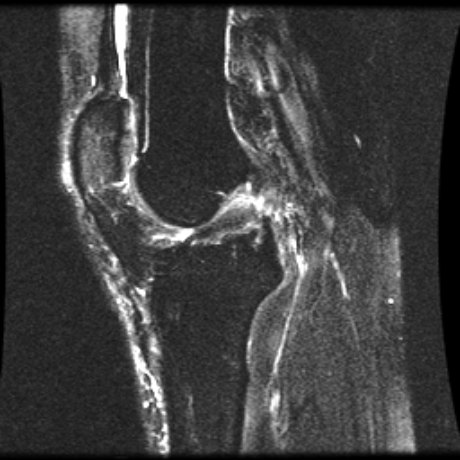
\includegraphics[width=\linewidth]{figs/plano_sagital.png}\\[2pt]\small Sagital\end{minipage}\hfill
\begin{minipage}{0.31\textwidth}\centering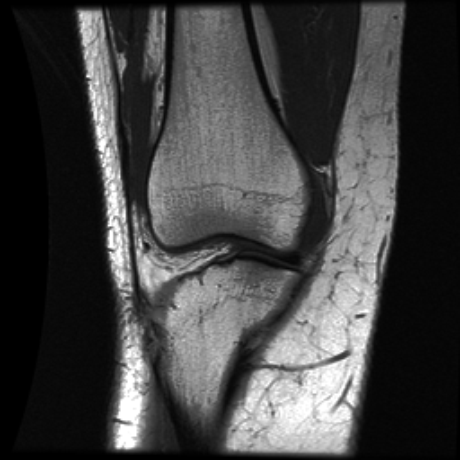
\includegraphics[width=\linewidth]{figs/plano_coronal.png}\\[2pt]\small Coronal\end{minipage}\hfill
\begin{minipage}{0.31\textwidth}\centering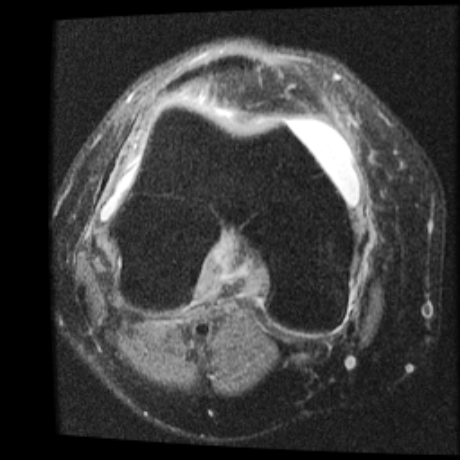
\includegraphics[width=\linewidth]{figs/plano_axial.png}\\[2pt]\small Axial\end{minipage}
\caption{Ejemplo de los tres planos anatómicos de un mismo estudio de RM de rodilla con rotura del LCA (MRNet).}
\label{fig:planos_ejemplo}
\end{figure}

Con el objetivo de evitar fuga de información (\textit{data leakage}), las particiones de entrenamiento, validación y prueba se realizaron a nivel de paciente.

\begin{table}[H]
\centering
\small
\caption{Distribución de casos clínicos empleados en el estudio.}
\label{tab:datos}
\begin{tabularx}{\textwidth}{
>{\raggedright\arraybackslash}X
>{\centering\arraybackslash}m{1.8cm}
>{\centering\arraybackslash}m{1.8cm}
>{\centering\arraybackslash}m{1.8cm}
>{\centering\arraybackslash}m{2cm}
}
\toprule
\textbf{Conjunto} &
\textbf{Casos} &
\textbf{LCA (+)} &
\textbf{Control (-)} &
\textbf{Prevalencia} \\
\midrule

Entrenamiento &
875 &
183 &
692 &
20.91\% \\

Validación &
188 &
36 &
152 &
19.15\% \\

Prueba &
187 &
43 &
144 &
22.99\% \\

\midrule
\textbf{Total} &
\textbf{1250} &
\textbf{262} &
\textbf{988} &
\textbf{20.96\%} \\

\bottomrule
\end{tabularx}
\end{table}

La distribución de clases presenta un desbalance considerable, reflejando una situación representativa del entorno clínico real, donde las lesiones completas del LCA representan una proporción minoritaria respecto al total de estudios de RM de rodilla.

\subsection{Conjunto externo de Croacia}

Además de MRNet, se utilizó un conjunto externo de resonancias magnéticas de rodilla procedente del Hospital Clínico Universitario de Rijeka (Croacia), publicado por {\v{S}}tajduhar et al.\ \cite{stajduhar2017semi}. Este conjunto permitió evaluar la robustez de los modelos ante un cambio de dominio, es decir, ante posibles diferencias en población, protocolo de adquisición, escáner o distribución de las imágenes respecto al conjunto original.

El conjunto de Croacia contiene 917 estudios. A diferencia de MRNet, su anotación original distingue tres grados de afectación del LCA: ligamento intacto (690 estudios), parcialmente roto (172 estudios) y completamente roto (55 estudios). Dado que en este trabajo la tarea se formula como una clasificación binaria (presencia o ausencia de rotura), las categorías de rotura parcial y rotura completa se unificaron en una única clase positiva, resultando en 690 casos sin rotura y 227 casos con rotura. Esta decisión sigue el criterio empleado por los propios autores del conjunto \cite{stajduhar2017semi} y permite una comparación directa con el etiquetado binario de MRNet, si bien debe tenerse en cuenta que la inclusión de roturas parciales introduce casos de mayor sutileza diagnóstica en la clase positiva. En primer lugar, se empleó para una validación externa \textit{zero-shot}, evaluando los modelos entrenados sobre MRNet sin reajustar sus pesos. Posteriormente, se utilizó para un experimento de \textit{fine-tuning} con el objetivo de analizar si la adaptación al nuevo dominio podía mejorar el rendimiento o modificar la calibración del clasificador.

Para el experimento de adaptación de dominio, el conjunto de Croacia se dividió en 641 casos de entrenamiento, 138 de validación y 138 de prueba. En el subconjunto de prueba había 104 casos sin rotura y 34 casos con rotura del LCA. Igual que en MRNet, las particiones se realizaron a nivel de paciente para evitar fuga de información entre conjuntos.

\section{Representación y preprocesamiento de datos}

Cada estudio de RM puede representarse matemáticamente como un volumen tridimensional:

\begin{equation}
V \in \mathbb{R}^{S \times H \times W}
\end{equation}

\noindent donde $S$ representa el número de cortes del volumen, mientras que $H$ y $W$ corresponden a la resolución espacial de cada corte.

Las intensidades de píxel fueron normalizadas mediante escalado Min-Max:

\begin{equation}
x_{\text{norm}} =
\frac{x - x_{\text{min}}}
{x_{\text{max}} - x_{\text{min}}}
\end{equation}

Posteriormente, todas las imágenes fueron redimensionadas a una resolución espacial de $224 \times 224$ píxeles. Dado que los modelos empleados utilizan pesos preentrenados en ImageNet, las imágenes monocanal fueron replicadas sobre tres canales de entrada.
\label{cap:metodologia}

\section{Descripción general del sistema}

El objetivo principal de este trabajo consiste en desarrollar un sistema de aprendizaje profundo capaz de detectar automáticamente lesiones del ligamento cruzado anterior (LCA) a partir de estudios de resonancia magnética (RM) de rodilla.

La metodología propuesta sigue un enfoque de clasificación directa de extremo a extremo (\textit{end-to-end}), evitando etapas explícitas de segmentación anatómica. Esta decisión se fundamenta tanto en criterios prácticos como clínicos. Por una parte, los modelos de segmentación requieren máscaras anotadas manualmente por especialistas, lo que supone un elevado coste temporal y computacional. Por otra, la clasificación directa permite preservar información contextual relevante de toda la articulación, incluyendo signos indirectos de lesión.

El pipeline general desarrollado puede dividirse en las siguientes etapas:

\begin{enumerate}
    \item Carga y normalización de estudios de resonancia magnética.
    \item Selección automática de cortes anatómicamente relevantes.
    \item Extracción de características mediante arquitecturas CNN y Transformer.
    \item Agregación de información entre cortes utilizando mecanismos de atención.
    \item Fusión multi-vista entre planos anatómicos.
    \item Clasificación binaria de lesión del LCA.
\end{enumerate}

La Figura~\ref{fig:pipeline_general} resume gráficamente este flujo de procesamiento, desde el volumen de RM de entrada hasta la predicción final de lesión del LCA.

\begin{figure}[H]
\centering
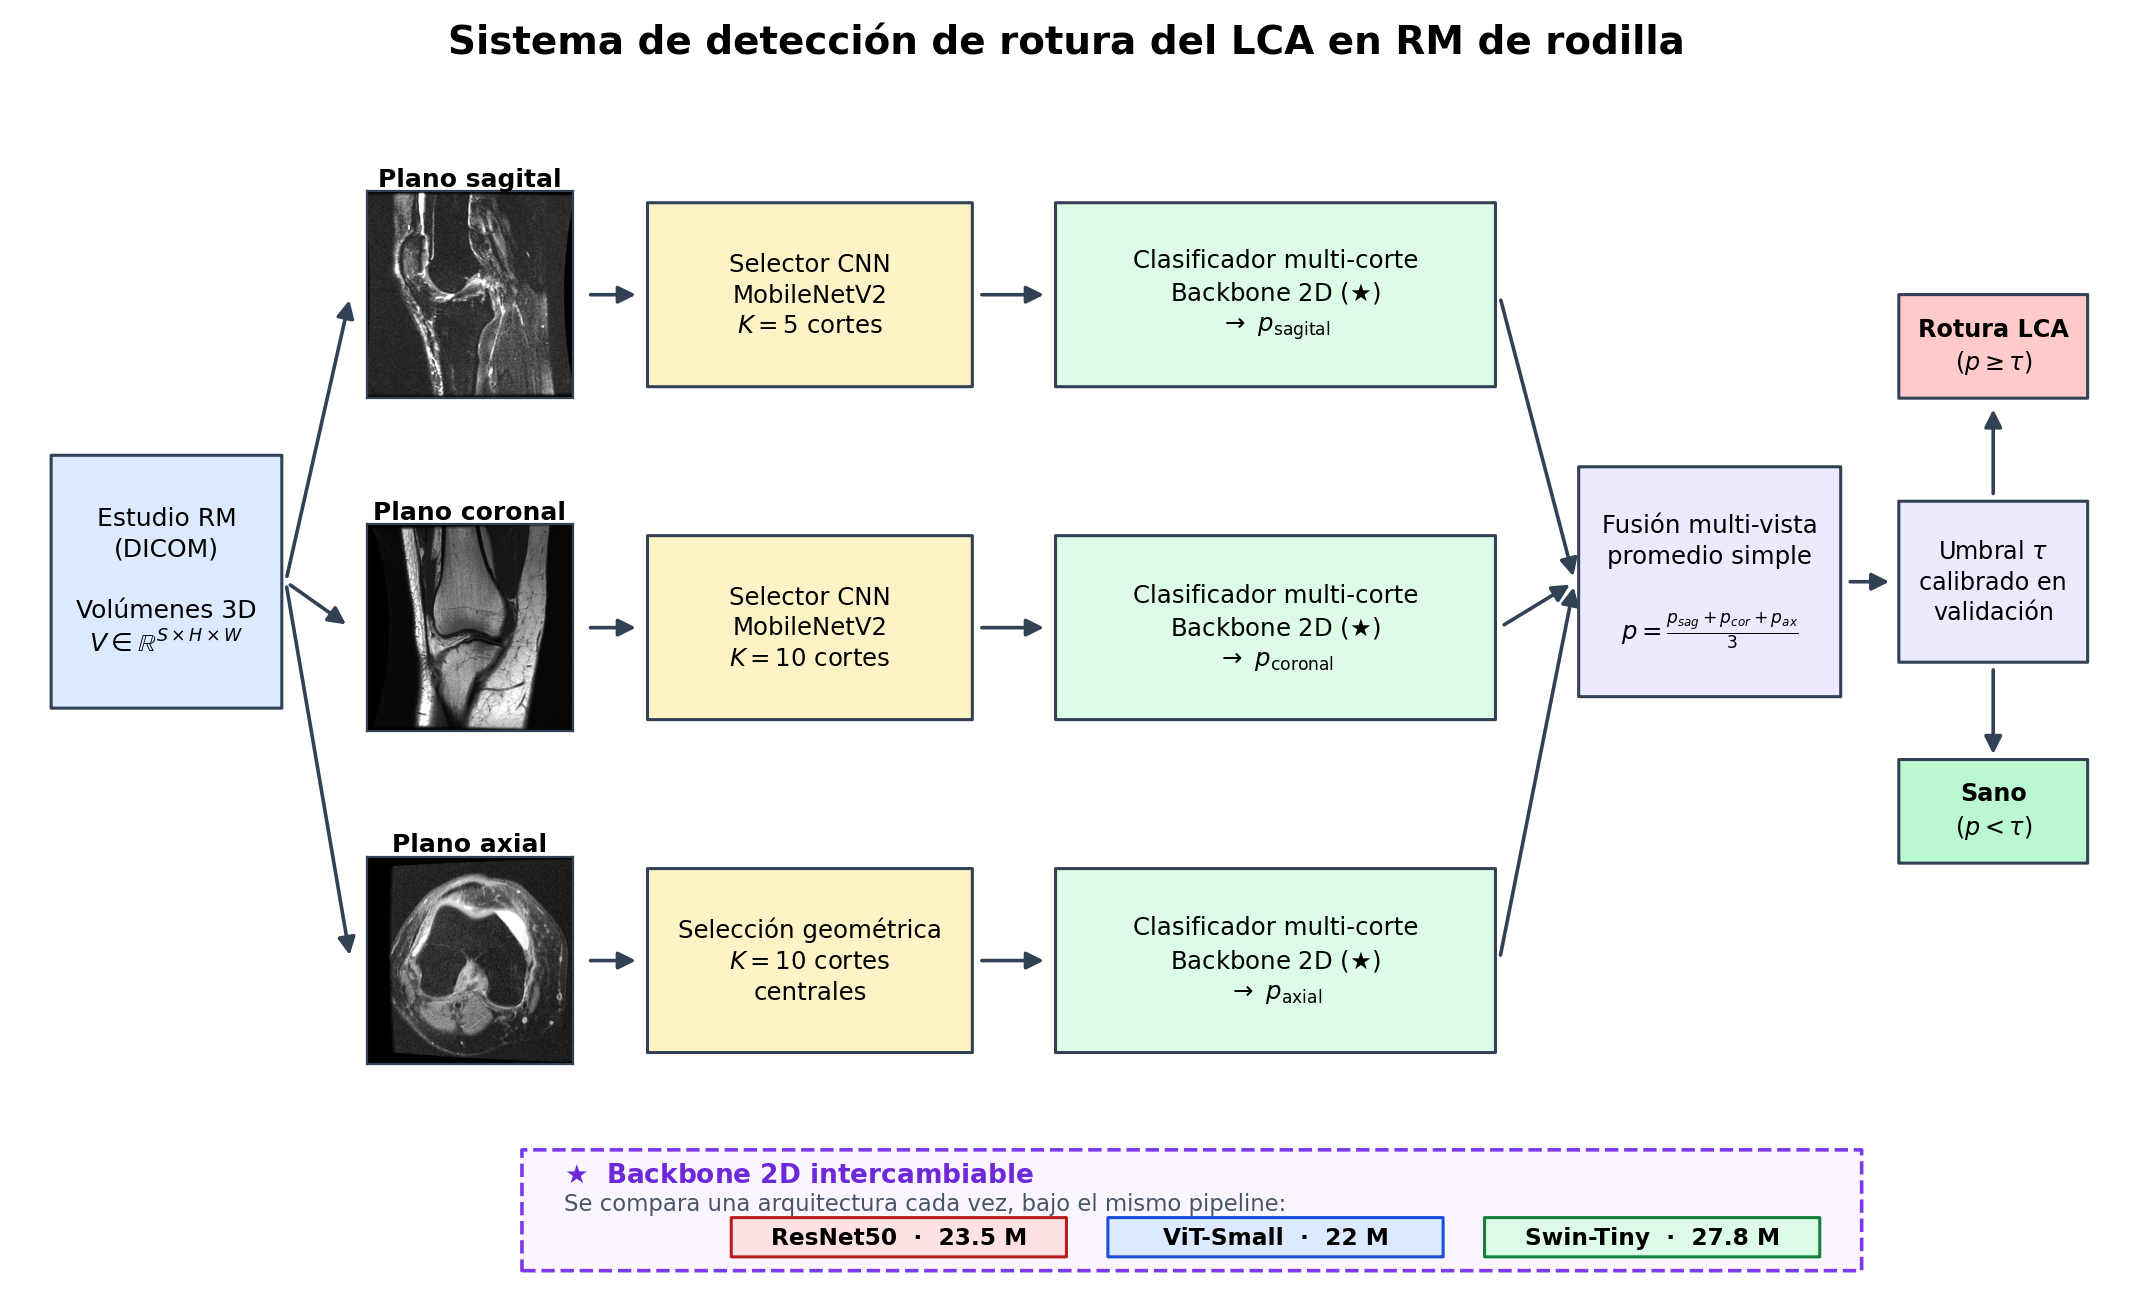
\includegraphics[width=0.92\textwidth]{figs/pipeline_general.png}
\caption{Esquema general del sistema propuesto: selección automática de cortes por plano, extracción de características mediante el \textit{backbone}, agregación de cortes mediante \textit{Attention Pooling} y fusión multi-vista de los tres planos anatómicos.}
\label{fig:pipeline_general}
\end{figure}

\section{Selección automática de cortes anatómicos}

Uno de los principales problemas asociados al procesamiento completo de volúmenes de RM es que únicamente una fracción reducida de los cortes contiene información anatómica relevante sobre el ligamento cruzado anterior.

Procesar todos los cortes incrementa:
\begin{itemize}
    \item el ruido visual,
    \item el coste computacional,
    \item y la redundancia espacial.
\end{itemize}

Por este motivo, en este trabajo se desarrolló un módulo propio de selección automática de cortes basado en una arquitectura \textbf{MobileNetV2}. En concreto, se entrenaron dos modelos independientes: uno específico para el plano sagital y otro específico para el plano coronal. Cada uno de ellos fue entrenado con sus propias etiquetas de relevancia anatómica, generadas de forma independiente para el plano correspondiente, de modo que el selector aprendiera qué cortes eran más informativos dentro de cada orientación.

La idea principal consiste en procesar los $N$ cortes que componen una serie de resonancia magnética y asignar a cada uno de ellos una puntuación de probabilidad asociada a la presencia o visibilidad del LCA en la imagen. A partir de estas puntuaciones, el sistema ordena los cortes de mayor a menor relevancia anatómica y selecciona automáticamente los $K$ cortes más informativos para el clasificador final.

De este modo, para cada estudio de RM el módulo actúa como una etapa previa de filtrado: recibe una secuencia completa de cortes sagitales o coronales y devuelve únicamente los 5 o 10 cortes con mayor probabilidad de contener información útil sobre el LCA, según el plano anatómico considerado. Esta selección no pretende diagnosticar la lesión, sino localizar las imágenes donde el ligamento es más visible o donde es más probable que aparezca información anatómica relevante para la clasificación posterior.

Esta estrategia se plantea como una contribución metodológica específica del trabajo. En lugar de utilizar únicamente cortes centrales o procesar todo el volumen completo, se introduce un selector aprendido que reduce la redundancia, limita el ruido visual y concentra el entrenamiento de los modelos diagnósticos en las regiones más relevantes. Hasta donde se ha revisado en el desarrollo de este trabajo, no se ha identificado una estrategia equivalente aplicada de esta forma en los trabajos comparados.

La Figura~\ref{fig:mri_slices_sagital} muestra un ejemplo real de los cortes sagitales seleccionados por el módulo para un estudio de RM, ordenados según la puntuación de relevancia anatómica asignada por el selector.

\begin{figure}[H]
\centering
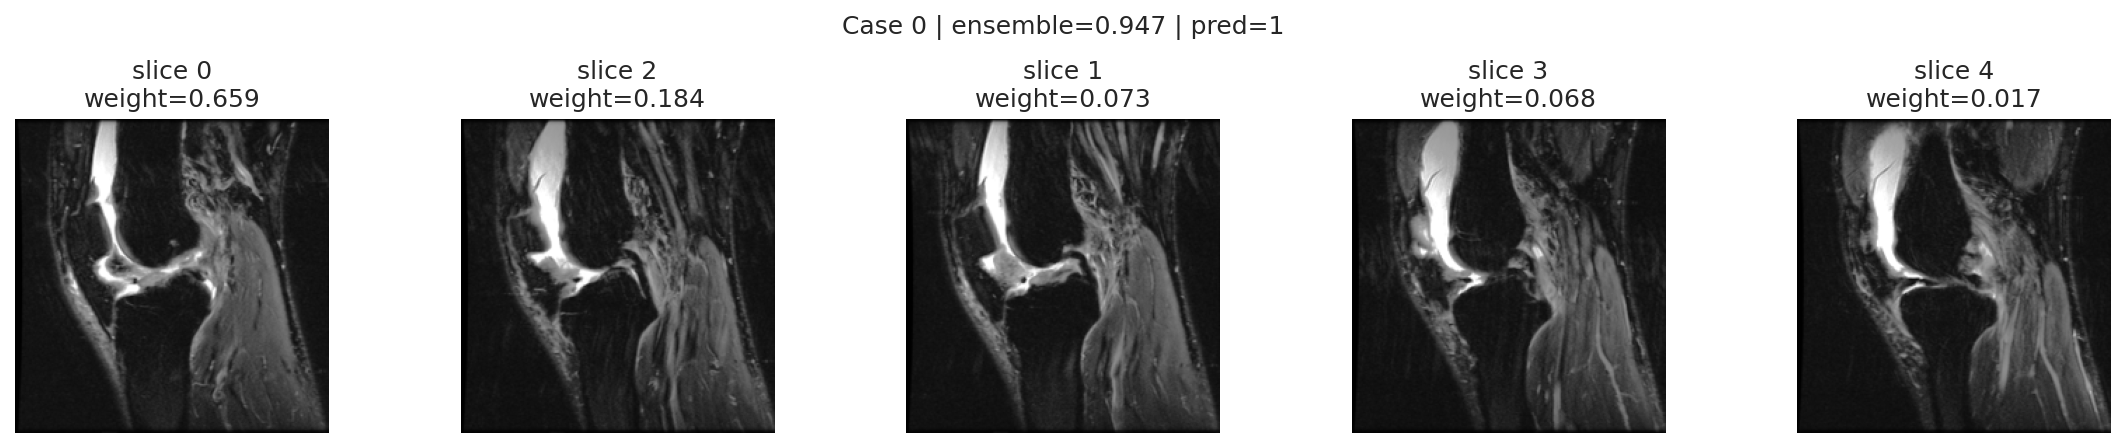
\includegraphics[width=\textwidth]{figs/mri_slices_sagital.png}
\caption{Ejemplo de cortes sagitales de un estudio de RM de rodilla seleccionados automáticamente por el módulo MobileNetV2, ordenados de mayor a menor probabilidad de contener información relevante del LCA.}
\label{fig:mri_slices_sagital}
\end{figure}

\subsection{Estrategias evaluadas}

Se analizaron distintas estrategias de selección:

\begin{itemize}
    \item \textbf{Center}: selección geométrica de los cortes centrales del volumen.
    \item \textbf{Random}: selección aleatoria utilizada durante entrenamiento como mecanismo de regularización.
    \item \textbf{CNN-Based}: selección automática basada en las puntuaciones generadas por MobileNetV2.
\end{itemize}

La configuración final utilizada fue:

\begin{itemize}
    \item Plano sagital: $K=5$ cortes mediante estrategia \textit{CNN-Based}.
    \item Plano coronal: $K=10$ cortes mediante estrategia \textit{CNN-Based}.
    \item Plano axial: $K=10$ cortes centrales consecutivos.
\end{itemize}

\section{Arquitecturas de aprendizaje profundo}

Con el objetivo de comparar distintos paradigmas de visión por computador, se seleccionaron arquitecturas representativas tanto de redes convolucionales como de Vision Transformers.

\begin{table}[H]
\centering
\small
\caption{Arquitecturas de aprendizaje profundo evaluadas en el estudio.}
\label{tab:modelos}
\begin{tabularx}{\textwidth}{
>{\raggedright\arraybackslash}X
>{\raggedright\arraybackslash}m{3cm}
>{\centering\arraybackslash}m{2cm}
}
\toprule
\textbf{Modelo} &
\textbf{Familia} &
\textbf{Parámetros} \\
\midrule

ResNet50 &
CNN residual &
23.5 M \\

ViT-Small &
Transformer global &
22.0 M \\

Swin-Tiny &
Transformer jerárquico &
27.8 M \\

\bottomrule
\end{tabularx}
\end{table}

Todas las arquitecturas comparten una misma cabeza de clasificación multi-corte: cada uno de los $K$ cortes seleccionados se procesa de forma independiente por el \textit{backbone} correspondiente, y los vectores de características resultantes se combinan mediante un mecanismo de \textit{Attention Pooling} que aprende a ponderar la importancia relativa de cada corte, produciendo un único vector de características ponderado para la clasificación. Por estar las tres arquitecturas diseñadas originalmente para imágenes bidimensionales, todas adoptan esta misma estrategia multi-corte para adaptarse al análisis volumétrico de la RM.

\section{Protocolo de entrenamiento y regularización}
\label{sec:protocolo_entrenamiento}

Las tres arquitecturas se entrenaron bajo un mismo protocolo, ajustando únicamente los valores específicos de cada modelo y plano anatómico. En todos los casos se empleó el optimizador \textbf{AdamW} con una fase inicial de calentamiento progresivo (\textit{warmup}) y un planificador dinámico de la tasa de aprendizaje ---por reducción ante meseta (\textit{ReduceLROnPlateau}) o por decaimiento tipo \textit{Cosine Annealing}, según la arquitectura---. Para estabilizar la optimización se aplicó recorte de gradientes (\textit{Gradient Clipping}) en los planos más propensos a oscilaciones.

Como técnicas de regularización comunes se utilizaron \textit{Dropout} (sobre la proyección de entrada del clasificador y sobre las capas densas), \textit{Label Smoothing} para evitar predicciones excesivamente confiadas y \textit{Early Stopping} monitorizando el AUC de validación. Estos parámetros se ajustaron de forma independiente para cada arquitectura y plano anatómico, en función de su sensibilidad al sobreajuste; los valores concretos se detallan en las tablas de cada modelo.

\section{Redes Convolucionales}
\label{sec:redes_convolucionales}

\subsection{ResNet50}
\label{subsec:cnn_resnet50}

El modelo \textit{Residual Network 50} (ResNet50) \cite{he2016deep} representa la arquitectura convolucional profunda utilizada como línea base en este trabajo. Esta arquitectura se fundamenta en el uso de conexiones residuales (\textit{skip connections}) que permiten facilitar la propagación del gradiente a través de las capas profundas:

\begin{equation}
y = \mathcal{F}(x, \{W_i\}) + x
\end{equation}

donde $x$ e $y$ representan los vectores de entrada y salida del bloque residual, mientras que $\mathcal{F}$ corresponde al mapeo residual aprendido por las capas convolucionales.

A diferencia de los modelos basados en Transformers, las redes convolucionales explotan de forma natural los sesgos inductivos de localidad espacial e invarianza a la traslación mediante el uso de filtros convolucionales compartidos. Esta propiedad las hace especialmente eficaces para detectar:
\begin{itemize}
    \item texturas locales,
    \item discontinuidades anatómicas,
    \item y patrones geométricos finos presentes en las fibras ligamentarias.
\end{itemize}

\subsubsection{Configuración y entrenamiento}

La configuración utilizada corresponde a ResNet50 preentrenada sobre ImageNet-1K (aproximadamente 23.5 millones de parámetros). Siguiendo la estrategia multi-corte común, la agregación entre cortes se realizó mediante \textit{Attention Pooling} en los planos sagital y axial, y mediante \textit{Max Pooling} en el coronal. El entrenamiento empleó el planificador \textit{ReduceLROnPlateau} junto con recorte de gradientes en los planos correspondientes. La Tabla~\ref{tab:regularizacion_cnn} recoge los parámetros de regularización por plano.

\begin{table}[H]
\centering
\small
\caption{Parámetros de regularización utilizados durante el entrenamiento de ResNet50.}
\label{tab:regularizacion_cnn}
\begin{tabularx}{\textwidth}{
>{\raggedright\arraybackslash}m{2.2cm}
>{\centering\arraybackslash}m{2cm}
>{\centering\arraybackslash}m{2cm}
>{\centering\arraybackslash}m{2.2cm}
>{\centering\arraybackslash}X
}
\toprule
\textbf{Plano} &
\textbf{Dropout Input} &
\textbf{Dropout Dense} &
\textbf{Label Smoothing} &
\textbf{Early Stopping} \\
\midrule

Sagital &
0.42 &
0.32 &
0.17 &
12 épocas \\

Coronal &
0.47 &
0.37 &
0.22 &
10 épocas \\

Axial &
0.42 &
0.32 &
0.17 &
12 épocas \\

\bottomrule
\end{tabularx}
\end{table}

\section{Vision Transformers}
\label{sec:vision_transformers}

\subsection{ViT-Small}
\label{subsec:vit_base}

El modelo \textit{Vision Transformer} (ViT) \cite{dosovitskiy2020image} reemplaza las convoluciones tradicionales por mecanismos de autoatención global. La imagen de entrada se divide inicialmente en pequeños parches bidimensionales:

\begin{equation}
x \rightarrow \{p_1, p_2, \dots, p_n\}
\end{equation}

Cada parche es proyectado posteriormente a un espacio de embeddings y procesado mediante bloques Transformer. El mecanismo de atención se calcula como:

\begin{equation}
\text{Attention}(Q,K,V) =
\text{softmax}
\left(
\frac{QK^T}{\sqrt{d_k}}
\right)V
\end{equation}

donde $Q$, $K$ y $V$ representan las matrices de consultas, claves y valores.

A diferencia de las redes convolucionales, el ViT permite modelar relaciones espaciales globales entre regiones anatómicas alejadas de la imagen mediante mecanismos de autoatención multi-cabeza (\textit{Multi-Head Self-Attention}, MHSA).

\subsubsection{Configuración y entrenamiento}

Como representante de la familia de transformers globales se empleó la variante \texttt{ViT-Small Patch16-224} (12 bloques Transformer, dimensión de embedding de 384, 6 cabezas de atención y aproximadamente 22 millones de parámetros). La elección de la variante \textit{Small} en lugar de la \textit{Base} (86 M) se justifica en la Sección~\ref{subsec:efecto_tamano}, donde se muestra que el aumento de capacidad no mejora el rendimiento en este problema. La agregación multi-corte se realizó mediante \textit{Attention Pooling} en los planos sagital y axial, y \textit{Max Pooling} en el coronal. El entrenamiento utilizó una tasa de aprendizaje máxima de $\eta_{\text{max}} = 1.2 \times 10^{-4}$ con \textit{warmup} seguido de decaimiento tipo \textit{Cosine Annealing}. La Tabla~\ref{tab:regularizacion_vit} detalla los parámetros de regularización por plano.

\begin{table}[H]
\centering
\small
\caption{Parámetros de regularización utilizados durante el entrenamiento de ViT-Small.}
\label{tab:regularizacion_vit}
\begin{tabularx}{\textwidth}{
>{\raggedright\arraybackslash}m{2.2cm}
>{\centering\arraybackslash}m{2cm}
>{\centering\arraybackslash}m{2cm}
>{\centering\arraybackslash}m{2.2cm}
>{\centering\arraybackslash}X
}
\toprule
\textbf{Plano} &
\textbf{Dropout Input} &
\textbf{Dropout Dense} &
\textbf{Label Smoothing} &
\textbf{Early Stopping} \\
\midrule

Sagital &
0.20 &
0.15 &
0.025 &
25 épocas \\

Coronal &
0.25 &
0.15 &
0.025 &
15 épocas \\

Axial &
0.25 &
0.15 &
0.05 &
15 épocas \\

\bottomrule
\end{tabularx}
\end{table}


\section{Swin Transformers}

\subsection{Swin-Tiny}
\label{subsec:swin_small}

El modelo \textit{Shifted Window Transformer Tiny} (Swin-Tiny) \cite{liu2021swin} representa una evolución jerárquica de los Vision Transformers basada en mecanismos de atención local mediante ventanas desplazadas (\textit{Shifted Window Self-Attention}).

A diferencia de Vision Transformer (ViT), donde la atención se calcula globalmente entre todos los parches de la imagen, Swin Transformer restringe el cálculo de atención a ventanas locales no solapadas, reduciendo significativamente la complejidad computacional.

El mecanismo de atención puede expresarse como:

\begin{equation}
\text{Attention}(Q,K,V) =
\text{softmax}
\left(
\frac{QK^T}{\sqrt{d_k}} + B
\right)V
\end{equation}

donde $B$ representa una matriz de sesgo de posición relativa que codifica la distancia espacial entre los parches dentro de cada ventana.

Mediante la estrategia de ventanas desplazadas, el modelo permite el intercambio progresivo de información contextual entre regiones vecinas de la imagen, combinando eficiencia computacional y capacidad de representación multiescala.

\subsubsection{Configuración y entrenamiento}

La configuración corresponde a la variante \texttt{swin\_tiny\_patch4\_window7\_224} preentrenada sobre ImageNet-1K (aproximadamente 27.8 millones de parámetros, organizados en cuatro etapas jerárquicas con profundidades de bloques $[2,2,6,2]$ y dimensión de embedding inicial de 96), con entrada de $224 \times 224$ píxeles. La arquitectura procesa parches iniciales de $4 \times 4$ píxeles y construye representaciones jerárquicas mediante operaciones de \textit{Patch Merging}. A diferencia de ResNet50 y ViT-Small, la agregación multi-corte se realizó mediante \textit{Attention Pooling} en los tres planos. El entrenamiento empleó una tasa de aprendizaje inicial de $1.3 \times 10^{-4}$ con \textit{ReduceLROnPlateau} (factor de reducción $0.5$) y recorte de gradientes con norma límite $1.0$. En el plano axial, el \textit{dropout input} se fijó en 0.00 para preservar las características visuales finas del LCA en la representación transversal, mientras que los planos sagital y coronal emplearon mayor regularización por su mayor redundancia anatómica. La Tabla~\ref{tab:regularizacion_swin} recoge los valores por plano.

\begin{table}[H]
\centering
\small
\caption{Parámetros de regularización utilizados durante el entrenamiento de Swin-Tiny.}
\label{tab:regularizacion_swin}
\begin{tabularx}{\textwidth}{
>{\raggedright\arraybackslash}m{2.2cm}
>{\centering\arraybackslash}m{2.0cm}
>{\centering\arraybackslash}m{2.0cm}
>{\centering\arraybackslash}m{2.2cm}
>{\centering\arraybackslash}X
}
\toprule
\textbf{Plano} &
\textbf{Dropout Input} &
\textbf{Dropout Dense} &
\textbf{Label Smoothing} &
\textbf{Early Stopping} \\
\midrule

Sagital &
0.42 &
0.32 &
0.17 &
12 épocas \\

Coronal &
0.42 &
0.32 &
0.17 &
40 épocas \\

Axial &
0.00 &
0.20 &
0.05 &
30 épocas \\

\bottomrule
\end{tabularx}
\end{table}

\chapter{Resultados y Discusión}
% -------------------------------------------------------------------------
% RESULTADOS Y DISCUSION
% Este archivo esta pensado para incluirse dentro del capitulo de resultados.
% No contiene comandos \chapter ni \section, y mantiene la estructura basada
% en \subsection y \subsubsection.
% -------------------------------------------------------------------------

\subsection{Diseño experimental y criterios de evaluación clínica}
\label{subsec:diseno_experimental_resultados}

El objetivo de los experimentos fue evaluar la capacidad de distintas arquitecturas de aprendizaje profundo para detectar roturas del ligamento cruzado anterior (LCA) en estudios de resonancia magnética de rodilla. Para ello, se compararon tres familias de modelos: una red convolucional residual, \textit{ResNet50}; un transformer global, \textit{Vision Transformer Small} (ViT-Small); y un transformer jerárquico basado en ventanas desplazadas, \textit{Swin Transformer Tiny}.

El entrenamiento se organizó por planos anatómicos. Se entrenaron modelos independientes para las proyecciones sagital, coronal y axial y, posteriormente, se integraron sus salidas probabilísticas en un ensamble multi-vista. Además, para cada arquitectura y plano anatómico se utilizaron diez semillas independientes, comprendidas entre la 42 y la 51, con el fin de cuantificar la estabilidad del entrenamiento.

La métrica prioritaria fue la sensibilidad o \textit{recall}, ya que un falso negativo implica no detectar una lesión real. Por ello, el umbral de decisión se seleccionó en validación maximizando la sensibilidad bajo una precisión mínima de 0.75:

\begin{equation}
\tau^* =
\operatorname*{arg\,max}_{\tau} \; \mathrm{Recall}(\tau)
\quad
\text{sujeto a}
\quad
\mathrm{Precision}(\tau) \geq 0.75 .
\label{eq:threshold_clinico}
\end{equation}

El suelo de precisión del 0.75 actúa como salvaguarda frente a la solución trivial de clasificar todos los estudios como positivos (que maximizaría la sensibilidad a costa de una precisión inaceptable), garantizando que al menos tres de cada cuatro casos señalados como positivos correspondan a roturas reales. La calibración del umbral se realizó exclusivamente sobre validación; el conjunto de test se utilizó solo para estimar el rendimiento final bajo el punto operativo seleccionado. En la Sección~\ref{subsec:discusion_general_resultados} se analiza la robustez de este umbral.

La combinación multi-vista se realizó mediante el promedio simple de las probabilidades obtenidas por los tres modelos especializados por plano:

\begin{equation}
\hat{p}_{\mathrm{ens}} =
\frac{
\hat{p}_{\mathrm{sagital}} +
\hat{p}_{\mathrm{coronal}} +
\hat{p}_{\mathrm{axial}}
}{3}.
\label{eq:ensemble_promedio}
\end{equation}

Este esquema de fusión no introduce parámetros adicionales y permite comparar directamente el rendimiento de modelos individuales y multi-vista.

\subsubsection{Hiperparámetros relevantes del entrenamiento}

En los experimentos multi-semilla se emplearon aumentos de datos, \textit{dropout}, suavizado de etiquetas cuando correspondía y \textit{early stopping} con paciencia máxima de 25 épocas.

Conviene aclarar un aspecto de interpretación de las curvas de entrenamiento. El criterio de parada se basa en el AUC de \textit{validación}, no en la pérdida de entrenamiento, y el modelo conservado en cada caso es el del \textbf{mejor AUC de validación}, no el de la última época. Por ello es esperable que la pérdida de entrenamiento aún muestre margen de descenso en el punto de corte: detenerse cuando la validación deja de mejorar evita precisamente el sobreajuste que supondría prolongar el entrenamiento. Las oscilaciones residuales de las curvas de validación reflejan el tamaño reducido del conjunto (188 estudios), lo que motiva el promediado multi-semilla.

El experimento de adaptación de dominio se realizó con el conjunto externo de Croacia descrito en el capítulo de materiales. En este caso, se ajustó el modelo Swin-Tiny sagital con una tasa de aprendizaje inicial de $2 \times 10^{-4}$, pérdida BCE ponderada con \texttt{pos\_weight} = 3.0314, \textit{dropout} de 0.3 en la entrada del clasificador y \textit{dropout} de 0.2 en la capa densa final.

% -------------------------------------------------------------------------
% RESULTADOS RESNET50
% -------------------------------------------------------------------------

\subsection{Resultados del modelo convolucional ResNet50}
\label{subsec:resultados_resnet50}

La arquitectura convolucional \textit{ResNet50} se utilizó como referencia frente a los modelos basados en transformers.

\subsubsection{Análisis de estabilidad multi-semilla}

La Tabla~\ref{tab:multiseed_resnet50} resume la estabilidad multi-semilla de ResNet50.

\begin{table}[H]
\centering
\small
\caption{Análisis de estabilidad multi-semilla para la arquitectura ResNet50.}
\label{tab:multiseed_resnet50}
\begin{tabularx}{\textwidth}{
>{\raggedright\arraybackslash}X
>{\centering\arraybackslash}m{1.8cm}
>{\centering\arraybackslash}m{1.8cm}
>{\centering\arraybackslash}m{1.8cm}
>{\centering\arraybackslash}m{1.8cm}
>{\centering\arraybackslash}m{1.8cm}
}
\toprule
\textbf{Plano} &
\textbf{AUC medio} &
\textbf{Desv. est.} &
\textbf{AUC mín.} &
\textbf{AUC máx.} &
\textbf{Mejor semilla} \\
\midrule
Sagital & 0.9425 & 0.0170 & 0.9132 & 0.9638 & 46 \\
Coronal & 0.9390 & 0.0169 & 0.8973 & 0.9638 & 44 \\
Axial   & \textbf{0.9610} & \textbf{0.0087} & \textbf{0.9501} & \textbf{0.9810} & \textbf{51} \\
\bottomrule
\end{tabularx}
\end{table}

El plano axial presentó simultáneamente el mayor AUC medio y la menor desviación estándar en validación, lo que indica un comportamiento particularmente estable. Los planos sagital y coronal también mostraron valores medios elevados, aunque con una variabilidad mayor entre ejecuciones. Esta diferencia refuerza la utilidad del análisis multi-semilla: una única ejecución podría sobreestimar o subestimar el rendimiento real de la arquitectura.

La Figura~\ref{fig:resnet_multiseed_training} muestra la evolución del entrenamiento multi-semilla de ResNet50 en los tres planos anatómicos.

\begin{figure}[H]
\centering

\includegraphics[width=0.88\textwidth]{figs/outputs/CNN_sagittal_entrenamiento_multiseed.png}

\vspace{0.6em}


\includegraphics[width=0.88\textwidth]{figs/outputs/CNN_coronal_entrenamiento_multiseed.png}

\vspace{0.6em}


\includegraphics[width=0.88\textwidth]{figs/outputs/CNN_axial_entrenamiento_multiseed.png}
\caption{Evolución del entrenamiento multi-semilla de ResNet50 en los planos sagital, coronal y axial.}
\label{fig:resnet_multiseed_training}
\end{figure}


\subsubsection{Rendimiento de los modelos fijados por validación por plano anatómico}

Tras el análisis multi-semilla, se fijó un checkpoint por plano anatómico utilizando únicamente el comportamiento observado en validación. El conjunto de test se empleó después solo como evaluación final. Estos resultados se resumen en la Tabla~\ref{tab:resnet_individual}.

\begin{table}[H]
\centering
\small
\caption{Rendimiento de los modelos ResNet50 fijados por plano anatómico utilizando únicamente validación.}
\label{tab:resnet_individual}
\begin{tabularx}{\textwidth}{
>{\raggedright\arraybackslash}X
>{\centering\arraybackslash}m{2.2cm}
>{\centering\arraybackslash}m{2.2cm}
}
\toprule
\textbf{Plano anatómico} &
\textbf{AUC validación} &
\textbf{AUC test} \\
\midrule
Sagital & 0.9501 & 0.8679 \\
Coronal & 0.9735 & 0.9246 \\
Axial   & 0.9704 & 0.9294 \\
\bottomrule
\end{tabularx}
\end{table}

En la evaluación final sobre test, el plano sagital obtuvo el menor rendimiento individual, mientras que el axial alcanzó el mayor AUC.

La Figura~\ref{fig:resnet_best_training} recoge las curvas de entrenamiento de los checkpoints finalmente fijados por validación para cada plano.

\begin{figure}[H]
\centering

\includegraphics[width=0.88\textwidth]{figs/outputs/CNN_sagittal_best.png}

\vspace{0.6em}


\includegraphics[width=0.88\textwidth]{figs/outputs/CNN_coronal_best.png}

\vspace{0.6em}


\includegraphics[width=0.88\textwidth]{figs/outputs/CNN_axial_best.png}
\caption{Curvas de entrenamiento de los mejores checkpoints de ResNet50 por plano anatómico.}
\label{fig:resnet_best_training}
\end{figure}

\subsubsection{Ensamble multi-vista calibrado}

El ensamble ResNet50 utilizó un umbral calibrado en validación de $\tau = 0.5445$. Sus métricas principales se recogen en la Tabla~\ref{tab:ensemble_resnet50_metricas}.

\begin{table}[H]
\centering
\scriptsize
\caption{Rendimiento del ensamble multi-vista basado en ResNet50 con umbral calibrado en validación.}
\label{tab:ensemble_resnet50_metricas}
\begin{tabularx}{\textwidth}{
>{\raggedright\arraybackslash}X
>{\centering\arraybackslash}m{1.15cm}
>{\centering\arraybackslash}m{1.15cm}
>{\centering\arraybackslash}m{1.15cm}
>{\centering\arraybackslash}m{1.15cm}
>{\centering\arraybackslash}m{1.15cm}
>{\centering\arraybackslash}m{1.15cm}
>{\centering\arraybackslash}m{1.15cm}
}
\toprule
\textbf{Conjunto} &
\textbf{AUC} &
\textbf{Acc} &
\textbf{Prec.} &
\textbf{Recall} &
\textbf{Esp.} &
\textbf{F1} &
\textbf{Umbral} \\
\midrule
Validación & 0.9836 & 0.9362 & 0.7609 & 0.9722 & 0.9276 & 0.8537 & 0.5445 \\
Test       & 0.9545 & 0.8556 & 0.6333 & 0.8837 & 0.8472 & 0.7379 & 0.5445 \\
\bottomrule
\end{tabularx}
\end{table}

\begin{table}[H]
\centering
\small
\caption{Matriz de confusión del ensamble ResNet50.}
\label{tab:ensemble_resnet50_confusion}
\begin{tabularx}{\textwidth}{
>{\raggedright\arraybackslash}X
>{\centering\arraybackslash}m{1.8cm}
>{\centering\arraybackslash}m{1.8cm}
>{\centering\arraybackslash}m{1.8cm}
>{\centering\arraybackslash}m{1.8cm}
}
\toprule
\textbf{Conjunto} &
\textbf{VP} &
\textbf{FN} &
\textbf{FP} &
\textbf{VN} \\
\midrule
Validación & 35 & 1 & 11 & 141 \\
Test       & 38 & 5 & 22 & 122 \\
\bottomrule
\end{tabularx}
\end{table}

En la evaluación final sobre test de MRNet, el ensamble ResNet50 alcanzó un AUC de 0.9545. Su sensibilidad fue ligeramente inferior a la obtenida por Swin-Tiny: ResNet50 dejó 5 falsos negativos en test, frente a los 4 falsos negativos del ensamble Swin-Tiny.

% -------------------------------------------------------------------------
% RESULTADOS VIT-SMALL
% -------------------------------------------------------------------------

\subsection{Resultados del modelo Vision Transformer (ViT-Small)}
\label{subsec:resultados_vitbase}

\textit{Vision Transformer Small} (ViT-Small) procesa la imagen como una secuencia de parches y emplea autoatención global, con una dimensión de \textit{embedding} de 384 y aproximadamente 22 millones de parámetros. Se adopta como representante de la familia de transformers globales por su mejor equilibrio entre rendimiento y coste; la comparación con la variante mayor ViT-Base se aborda específicamente en la Sección~\ref{subsec:efecto_tamano}.

\subsubsection{Análisis de estabilidad multi-semilla}

La Tabla~\ref{tab:multiseed_vitbase} presenta el análisis multi-semilla de ViT-Small para las diez semillas evaluadas.

\begin{table}[H]
\centering
\small
\caption{Análisis de estabilidad multi-semilla para la arquitectura ViT-Small.}
\label{tab:multiseed_vitbase}
\begin{tabularx}{\textwidth}{
>{\raggedright\arraybackslash}X
>{\centering\arraybackslash}m{1.8cm}
>{\centering\arraybackslash}m{1.8cm}
>{\centering\arraybackslash}m{1.8cm}
>{\centering\arraybackslash}m{1.8cm}
>{\centering\arraybackslash}m{1.8cm}
}
\toprule
\textbf{Plano} &
\textbf{AUC medio} &
\textbf{Desv. est.} &
\textbf{AUC mín.} &
\textbf{AUC máx.} &
\textbf{Mejor semilla} \\
\midrule
Sagital & 0.9621 & 0.0100 & 0.9404 & 0.9764 & 43 \\
Coronal & 0.8740 & 0.0512 & 0.8035 & 0.9377 & 51 \\
Axial   & 0.9525 & 0.0074 & 0.9437 & 0.9695 & 48 \\
\bottomrule
\end{tabularx}
\end{table}

El análisis multi-semilla evidencia una diferencia importante entre planos. Los planos axial y sagital fueron los más estables, con desviaciones estándar de 0.0074 y 0.0100 respectivamente, mientras que el plano coronal presentó una variabilidad superior (0.0512). Esta inestabilidad puede explicarse por la dificultad de localizar de forma consistente el LCA en dicha proyección, donde la estructura puede aparecer parcialmente representada y con mayor interferencia de tejidos circundantes. Aun así, esta variabilidad es notablemente menor que la observada en otras arquitecturas para el mismo plano.

La sensibilidad de ViT-Small a la inicialización es coherente con la naturaleza de los transformers globales. Al no incorporar de forma explícita el sesgo inductivo de localidad espacial característico de las redes convolucionales, el modelo debe aprender durante el entrenamiento qué relaciones entre parches son relevantes. Esta flexibilidad puede ser beneficiosa cuando la convergencia es adecuada, pero también puede incrementar la variabilidad en conjuntos médicos de tamaño moderado.

La Figura~\ref{fig:vit_multiseed_training} muestra la evolución del entrenamiento multi-semilla de ViT-Small en los tres planos anatómicos.

\begin{figure}[H]
\centering

\includegraphics[width=0.88\textwidth]{figs/outputs/VIT_sagittal_entrenamiento_multiseed.png}

\vspace{0.6em}


\includegraphics[width=0.88\textwidth]{figs/outputs/VIT_coronal_entrenamiento_multiseed.png}

\vspace{0.6em}


\includegraphics[width=0.88\textwidth]{figs/outputs/VIT_axial_entrenamiento_multiseed.png}
\caption{Evolución del entrenamiento multi-semilla de ViT-Small en los planos sagital, coronal y axial.}
\label{fig:vit_multiseed_training}
\end{figure}

\subsubsection{Rendimiento de los modelos fijados por validación por plano anatómico}

Tras el análisis multi-semilla, se fijó un modelo por plano utilizando únicamente la información de validación. Posteriormente, el conjunto de test se utilizó solo para estimar el rendimiento final. Los resultados se muestran en la Tabla~\ref{tab:vit_individual}.

\begin{table}[H]
\centering
\small
\caption{Rendimiento de los modelos ViT-Small fijados por plano anatómico utilizando únicamente validación.}
\label{tab:vit_individual}
\begin{tabularx}{\textwidth}{
>{\raggedright\arraybackslash}X
>{\centering\arraybackslash}m{2.2cm}
>{\centering\arraybackslash}m{2.2cm}
}
\toprule
\textbf{Plano anatómico} &
\textbf{AUC validación} &
\textbf{AUC test} \\
\midrule
Sagital & 0.9764 & 0.8932 \\
Coronal & 0.9377 & 0.8882 \\
Axial   & 0.9695 & 0.9380 \\
\bottomrule
\end{tabularx}
\end{table}

Los modelos fijados de ViT-Small alcanzaron un rendimiento competitivo en los tres planos. En validación destacaron los planos sagital y axial, mientras que las métricas de test se reportan exclusivamente como evaluación final.

\subsubsection{Ensamble multi-vista calibrado}

El ensamble ViT-Small utilizó un umbral de $\tau = 0.3804$, seleccionado en validación. La Tabla~\ref{tab:ensemble_vitbase_metricas} resume las métricas principales.

\begin{table}[H]
\centering
\scriptsize
\caption{Rendimiento del ensamble multi-vista basado en ViT-Small con umbral calibrado en validación.}
\label{tab:ensemble_vitbase_metricas}
\begin{tabularx}{\textwidth}{
>{\raggedright\arraybackslash}X
>{\centering\arraybackslash}m{1.15cm}
>{\centering\arraybackslash}m{1.15cm}
>{\centering\arraybackslash}m{1.15cm}
>{\centering\arraybackslash}m{1.15cm}
>{\centering\arraybackslash}m{1.15cm}
>{\centering\arraybackslash}m{1.15cm}
>{\centering\arraybackslash}m{1.15cm}
}
\toprule
\textbf{Conjunto} &
\textbf{AUC} &
\textbf{Acc} &
\textbf{Prec.} &
\textbf{Recall} &
\textbf{Esp.} &
\textbf{F1} &
\textbf{Umbral} \\
\midrule
Validación & 0.9837 & 0.9362 & 0.7500 & 1.0000 & 0.9211 & 0.8571 & 0.3804 \\
Test       & 0.9433 & 0.8663 & 0.6552 & 0.8837 & 0.8611 & 0.7525 & 0.3804 \\
\bottomrule
\end{tabularx}
\end{table}


\begin{table}[H]
\centering
\small
\caption{Matriz de confusión del ensamble ViT-Small.}
\label{tab:ensemble_vitbase_confusion}
\begin{tabularx}{\textwidth}{
>{\raggedright\arraybackslash}X
>{\centering\arraybackslash}m{1.8cm}
>{\centering\arraybackslash}m{1.8cm}
>{\centering\arraybackslash}m{1.8cm}
>{\centering\arraybackslash}m{1.8cm}
}
\toprule
\textbf{Conjunto} &
\textbf{VP} &
\textbf{FN} &
\textbf{FP} &
\textbf{VN} \\
\midrule
Validación & 36 & 0 & 12 & 140 \\
Test       & 38 & 5 & 20 & 124 \\
\bottomrule
\end{tabularx}
\end{table}

En validación, el ensamble ViT-Small detectó las 36 roturas presentes sin ningún falso negativo (sensibilidad de 1.0). En la evaluación final sobre test alcanzó un AUC de 0.9433 con 5 falsos negativos, mostrando un buen equilibrio entre sensibilidad y discriminación global.

La Figura~\ref{fig:vit_best_training} resume las curvas de mejores checkpoints de ViT-Small.

\begin{figure}[H]
\centering

\includegraphics[width=0.88\textwidth]{figs/outputs/VIT_sagittal_best.png}

\vspace{0.6em}


\includegraphics[width=0.88\textwidth]{figs/outputs/VIT_coronal_best.png}

\vspace{0.6em}


\includegraphics[width=0.88\textwidth]{figs/outputs/VIT_axial_best.png}
\caption{Curvas de entrenamiento de los mejores checkpoints de ViT-Small por plano anatómico.}
\label{fig:vit_best_training}
\end{figure}

% -------------------------------------------------------------------------
% RESULTADOS SWIN-SMALL
% -------------------------------------------------------------------------

\subsection{Resultados del modelo Swin Transformer Tiny}
\label{subsec:resultados_swin_small}

\textit{Swin Transformer Tiny} combina atención local mediante ventanas desplazadas con una representación jerárquica.

\subsubsection{Análisis de estabilidad multi-semilla}

Al igual que en ResNet50 y ViT-Small, Swin-Tiny fue evaluado mediante diez semillas independientes por plano anatómico. La Tabla~\ref{tab:multiseed_swin_small} resume los resultados de validación por plano.

\begin{table}[H]
\centering
\small
\caption{Análisis de estabilidad multi-semilla para la arquitectura Swin-Tiny.}
\label{tab:multiseed_swin_small}
\begin{tabularx}{\textwidth}{
>{\raggedright\arraybackslash}X
>{\centering\arraybackslash}m{2.0cm}
>{\centering\arraybackslash}m{2.0cm}
>{\centering\arraybackslash}m{2.0cm}
>{\centering\arraybackslash}m{2.0cm}
}
\toprule
\textbf{Plano} &
\textbf{AUC medio} &
\textbf{Desv. est.} &
\textbf{AUC mín.} &
\textbf{AUC máx.} \\
\midrule
Sagital & 0.9223 & 0.0787 & 0.7004 & 0.9649 \\
Coronal & 0.7748 & 0.1348 & 0.5970 & 0.9684 \\
Axial   & \textbf{0.9560} & \textbf{0.0123} & \textbf{0.9368} & \textbf{0.9722} \\
\bottomrule
\end{tabularx}
\end{table}

El plano axial fue el más estable, con un AUC medio de 0.9560 y una desviación estándar de 0.0123. En cambio, el plano coronal mostró la mayor variabilidad, con una desviación estándar de 0.1348 y un AUC mínimo de 0.5970, prácticamente equivalente al azar. Esto indica que, mientras algunas semillas alcanzaron un rendimiento elevado (AUC máximo de 0.9684), otras no llegaron a converger: el modelo colapsó hacia una solución trivial, próxima a predecir siempre la clase mayoritaria.

Este comportamiento puede explicarse por la conjunción de varios factores. Por una parte, el plano coronal es el más difícil para localizar el LCA de forma consistente, ya que el ligamento aparece a menudo parcialmente representado y con mayor interferencia de los tejidos circundantes; además, en este plano se procesan $K=10$ cortes, frente a los $5$ del sagital, lo que aumenta la proporción de información poco discriminativa. Por otra parte, la atención local por ventanas de Swin-Tiny depende de que la señal relevante esté espacialmente bien localizada; cuando la inicialización no consigue fijar esa señal débil en las primeras épocas, el entrenamiento queda atrapado en la solución trivial y no escapa de ella, de ahí los casos con AUC cercano a 0.5. Esta fragilidad refuerza la necesidad del análisis multi-semilla y justifica el papel del ensamble multi-vista, en el que la aportación más débil del plano coronal se compensa con la de los planos sagital y axial.

Por todo ello, la interpretación de Swin-Tiny debe basarse en el conjunto de evidencias: estabilidad en validación, comportamiento del ensamble y evaluación externa.

La Figura~\ref{fig:swin_multiseed_training} muestra la evolución del entrenamiento multi-semilla de Swin-Tiny en los tres planos anatómicos.

\begin{figure}[H]
\centering

\includegraphics[width=0.88\textwidth]{figs/outputs/SWIN_sagittal_entrenamiento_multiseed.png}

\vspace{0.6em}


\includegraphics[width=0.88\textwidth]{figs/outputs/SWIN_coronal_entrenamiento_multiseed.png}

\vspace{0.6em}


\includegraphics[width=0.88\textwidth]{figs/outputs/SWIN_axial_entrenamiento_multiseed.png}
\caption{Evolución del entrenamiento multi-semilla de Swin-Tiny en los planos sagital, coronal y axial.}
\label{fig:swin_multiseed_training}
\end{figure}

\subsubsection{Selección de modelos para el ensamble}

A partir del análisis multi-semilla se fijaron los checkpoints utilizados en cada plano anatómico para construir el ensamble, empleando únicamente información procedente de validación. De este modo, las métricas del ensamble no se presentan como una ejecución aislada, sino como el resultado de combinar modelos definidos antes de consultar el conjunto de test.

La Figura~\ref{fig:swin_best_training} recoge las curvas de entrenamiento de los checkpoints seleccionados para Swin-Tiny.

\begin{figure}[H]
\centering

\includegraphics[width=0.88\textwidth]{figs/outputs/SWIN_sagittal_best.png}

\vspace{0.6em}


\includegraphics[width=0.88\textwidth]{figs/outputs/SWIN_coronal_best.png}

\vspace{0.6em}


\includegraphics[width=0.88\textwidth]{figs/outputs/SWIN_axial_best.png}
\caption{Curvas de entrenamiento de los mejores checkpoints de Swin-Tiny por plano anatómico.}
\label{fig:swin_best_training}
\end{figure}

\subsubsection{Ensamble multi-vista calibrado}

El ensamble Swin-Tiny se construyó mediante promedio simple de las probabilidades de los tres planos. El umbral seleccionado en validación fue $\tau = 0.3734$. Las métricas se presentan en la Tabla~\ref{tab:ensemble_swin_metricas}.

\begin{table}[H]
\centering
\scriptsize
\caption{Rendimiento del ensamble multi-vista basado en Swin-Tiny con umbral calibrado en validación.}
\label{tab:ensemble_swin_metricas}
\begin{tabularx}{\textwidth}{
>{\raggedright\arraybackslash}X
>{\centering\arraybackslash}m{1.15cm}
>{\centering\arraybackslash}m{1.15cm}
>{\centering\arraybackslash}m{1.15cm}
>{\centering\arraybackslash}m{1.15cm}
>{\centering\arraybackslash}m{1.15cm}
>{\centering\arraybackslash}m{1.15cm}
>{\centering\arraybackslash}m{1.15cm}
}
\toprule
\textbf{Conjunto} &
\textbf{AUC} &
\textbf{Acc} &
\textbf{Prec.} &
\textbf{Recall} &
\textbf{Esp.} &
\textbf{F1} &
\textbf{Umbral} \\
\midrule
Validación & 0.9837 & 0.9362 & 0.7609 & 0.9722 & 0.9276 & 0.8537 & 0.3734 \\
Test       & 0.9536 & 0.8556 & 0.6290 & 0.9070 & 0.8403 & 0.7429 & 0.3734 \\
\bottomrule
\end{tabularx}
\end{table}


\begin{table}[H]
\centering
\small
\caption{Matriz de confusión del ensamble Swin-Tiny.}
\label{tab:ensemble_swin_confusion}
\begin{tabularx}{\textwidth}{
>{\raggedright\arraybackslash}X
>{\centering\arraybackslash}m{1.8cm}
>{\centering\arraybackslash}m{1.8cm}
>{\centering\arraybackslash}m{1.8cm}
>{\centering\arraybackslash}m{1.8cm}
}
\toprule
\textbf{Conjunto} &
\textbf{VP} &
\textbf{FN} &
\textbf{FP} &
\textbf{VN} \\
\midrule
Validación & 35 & 1 & 11 & 141 \\
Test       & 39 & 4 & 23 & 121 \\
\bottomrule
\end{tabularx}
\end{table}

En la evaluación final sobre test, Swin-Tiny obtuvo una sensibilidad de 0.9070, detectando 39 de las 43 roturas presentes y dejando 4 falsos negativos. El coste de este punto operativo fue un aumento de los falsos positivos, con 23 controles clasificados como positivos, lo que redujo su precisión y especificidad respecto a ViT-Small.

Desde una perspectiva clínica, este comportamiento puede ser favorable cuando se prioriza la reducción de falsos negativos. Sin embargo, no debe interpretarse como una mejora universal en todas las métricas ni como una elección definitiva basada en test.

% -------------------------------------------------------------------------
% COMPARATIVA FINAL EN MRNET
% -------------------------------------------------------------------------

\subsection{Comparativa final de ensambles en MRNet}
\label{subsec:comparativa_final_mrnet}

La comparación entre ensambles debe interpretarse separando dos niveles. En primer lugar, la Tabla~\ref{tab:comparativa_ensembles_mrnet_val} resume el rendimiento en validación, que es el conjunto utilizado para fijar los umbrales y describir el comportamiento operativo esperado. En segundo lugar, la Tabla~\ref{tab:comparativa_ensembles_mrnet_test} muestra la evaluación final sobre el conjunto de test de MRNet, utilizado únicamente para estimar la capacidad de generalización bajo las decisiones previamente fijadas.

Esta comparación permite distinguir entre rendimiento discriminativo global, medido mediante AUC, y rendimiento clínico bajo el umbral seleccionado, medido mediante sensibilidad, especificidad, precisión y F1-score.

\begin{table}[H]
\centering
\scriptsize
\caption{Comparativa de los ensambles multi-vista en el conjunto de validación de MRNet.}
\label{tab:comparativa_ensembles_mrnet_val}
\begin{tabularx}{\textwidth}{
>{\raggedright\arraybackslash}X
>{\centering\arraybackslash}m{1.05cm}
>{\centering\arraybackslash}m{1.05cm}
>{\centering\arraybackslash}m{1.05cm}
>{\centering\arraybackslash}m{1.05cm}
>{\centering\arraybackslash}m{1.05cm}
>{\centering\arraybackslash}m{1.05cm}
>{\centering\arraybackslash}m{1.05cm}
>{\centering\arraybackslash}m{1.05cm}
}
\toprule
\textbf{Modelo} &
\textbf{AUC} &
\textbf{Acc} &
\textbf{Prec.} &
\textbf{Recall} &
\textbf{Esp.} &
\textbf{F1} &
\textbf{FN} &
\textbf{FP} \\
\midrule
ViT-Small &
\textbf{0.9837} &
\textbf{0.9362} &
0.7500 &
\textbf{1.0000} &
0.9211 &
\textbf{0.8571} &
\textbf{0} &
12 \\

ResNet50 &
0.9836 &
\textbf{0.9362} &
\textbf{0.7609} &
0.9722 &
\textbf{0.9276} &
0.8537 &
1 &
\textbf{11} \\

Swin-Tiny &
\textbf{0.9837} &
\textbf{0.9362} &
\textbf{0.7609} &
0.9722 &
\textbf{0.9276} &
0.8537 &
1 &
\textbf{11} \\
\bottomrule
\end{tabularx}
\end{table}

\begin{table}[H]
\centering
\scriptsize
\caption{Comparativa de los ensambles multi-vista en el conjunto de test de MRNet.}
\label{tab:comparativa_ensembles_mrnet_test}
\begin{tabularx}{\textwidth}{
>{\raggedright\arraybackslash}X
>{\centering\arraybackslash}m{1.05cm}
>{\centering\arraybackslash}m{1.05cm}
>{\centering\arraybackslash}m{1.05cm}
>{\centering\arraybackslash}m{1.05cm}
>{\centering\arraybackslash}m{1.05cm}
>{\centering\arraybackslash}m{1.05cm}
>{\centering\arraybackslash}m{1.05cm}
>{\centering\arraybackslash}m{1.05cm}
}
\toprule
\textbf{Modelo} &
\textbf{AUC} &
\textbf{Acc} &
\textbf{Prec.} &
\textbf{Recall} &
\textbf{Esp.} &
\textbf{F1} &
\textbf{FN} &
\textbf{FP} \\
\midrule
ViT-Small &
0.9433 &
\textbf{0.8663} &
\textbf{0.6552} &
0.8837 &
\textbf{0.8611} &
\textbf{0.7525} &
5 &
\textbf{20} \\

ResNet50 &
\textbf{0.9545} &
0.8556 &
0.6333 &
0.8837 &
0.8472 &
0.7379 &
5 &
22 \\

Swin-Tiny &
0.9536 &
0.8556 &
0.6290 &
\textbf{0.9070} &
0.8403 &
0.7429 &
\textbf{4} &
23 \\
\bottomrule
\end{tabularx}
\end{table}

En validación, el ensamble ViT-Small alcanzó una sensibilidad perfecta (detectó las 36 roturas, sin falsos negativos), mientras que ResNet50 y Swin-Tiny obtuvieron un punto operativo con un falso negativo y once falsos positivos. En test, ResNet50 obtuvo el mayor AUC, ViT-Small mostró mayor exactitud, precisión, especificidad y F1-score, y Swin-Tiny alcanzó la mayor sensibilidad.

La Figura~\ref{fig:roc_ensembles_mrnet_val} agrupa las curvas ROC de validación de los tres ensambles, y la Figura~\ref{fig:roc_ensembles_mrnet_test} las correspondientes al conjunto de test, para las tres arquitecturas evaluadas.

\begin{figure}[H]
\centering
\begin{minipage}{0.32\textwidth}\centering

\includegraphics[width=\linewidth]{figs/outputs/CNN_ROC.png}
\end{minipage}\hfill
\begin{minipage}{0.32\textwidth}\centering

\includegraphics[width=\linewidth]{figs/outputs/VIT_ROC_val.png}
\end{minipage}\hfill
\begin{minipage}{0.32\textwidth}\centering

\includegraphics[width=\linewidth]{figs/outputs/SWIN_ROC_val.png}
\end{minipage}
\caption{Curvas ROC de validación de los ensambles ResNet50, ViT-Small y Swin-Tiny en MRNet.}
\label{fig:roc_ensembles_mrnet_val}
\end{figure}

\begin{figure}[H]
\centering
\begin{minipage}{0.32\textwidth}\centering

\includegraphics[width=\linewidth]{figs/outputs/CNN_ROC_test.png}
\end{minipage}\hfill
\begin{minipage}{0.32\textwidth}\centering

\includegraphics[width=\linewidth]{figs/outputs/VIT_ROC_test.png}
\end{minipage}\hfill
\begin{minipage}{0.32\textwidth}\centering

\includegraphics[width=\linewidth]{figs/outputs/SWIN_ROC_test.png}
\end{minipage}
\caption{Curvas ROC de test de los ensambles ResNet50, ViT-Small y Swin-Tiny en MRNet.}
\label{fig:roc_ensembles_mrnet_test}
\end{figure}

En consecuencia, no se propone una selección definitiva de un único modelo a partir del conjunto de test. La comparación en validación permite justificar el comportamiento operativo sin usar test para tomar decisiones, mientras que la comparación en test permite describir compromisos finales entre discriminación global, sensibilidad y falsos positivos.

% -------------------------------------------------------------------------
% FALSOS NEGATIVOS COMUNES
% -------------------------------------------------------------------------

\subsection{Análisis de los falsos negativos comunes a las tres arquitecturas}
\label{subsec:falsos_negativos_comunes}

Un falso negativo, es decir, un estudio con rotura real del LCA clasificado como sano, constituye el error más relevante en este dominio clínico, pues implica no detectar una lesión presente. Para comprender la naturaleza de los errores residuales del sistema se analizaron los falsos negativos compartidos por las tres arquitecturas, bajo la hipótesis de que un caso que los tres modelos ---entrenados de forma independiente y con \textit{backbones} de naturaleza muy distinta--- clasifican erróneamente en el mismo sentido difícilmente se explica por una limitación particular de una arquitectura concreta.

Del conjunto de test de MRNet, únicamente tres estudios fueron clasificados como negativos por los tres ensambles de forma simultánea: los casos 0080, 0087 y 0521. La Tabla~\ref{tab:fn_comunes} recoge las probabilidades asignadas por cada arquitectura a estos tres casos.

\begin{table}[H]
\centering
\small
\caption{Probabilidad de rotura asignada por cada ensamble a los tres falsos negativos comunes del conjunto de test. La etiqueta real de los tres casos es rotura del LCA (positivo).}
\label{tab:fn_comunes}
\begin{tabularx}{\textwidth}{
>{\centering\arraybackslash}X
>{\centering\arraybackslash}X
>{\centering\arraybackslash}X
>{\centering\arraybackslash}X
}
\toprule
\textbf{Caso} &
\textbf{ResNet50} &
\textbf{ViT-Small} &
\textbf{Swin-Tiny} \\
\midrule
0080 & 0.3805 & 0.0630 & 0.2473 \\
0087 & 0.5338 & 0.1054 & 0.3115 \\
0521 & 0.4899 & 0.2548 & 0.2708 \\
\bottomrule
\end{tabularx}
\end{table}

Las probabilidades asignadas son sistemáticamente bajas, especialmente en el caso de ViT-Small, lo que indica que los modelos no se encuentran ante una decisión dudosa próxima al umbral, sino que la evidencia visual de rotura captada por las redes es escasa. La coincidencia de los tres modelos en estos mismos casos sugiere que no se trata de errores estocásticos asociados a una inicialización o arquitectura particular, sino de estudios intrínsecamente difíciles.

Para cuantificar el impacto de estos tres casos, se recalculó el AUC de test bajo el supuesto de que correspondieran realmente a estudios sin rotura ---es decir, asumiendo la hipótesis de un posible etiquetado incorrecto---. Bajo este supuesto, el AUC aumentaría de 0.9433 a 0.9794 en ViT-Small (un incremento de 0.0361, el mayor de los tres), de 0.9536 a 0.9774 en Swin-Tiny ($+$0.0237) y de 0.9545 a 0.9675 en ResNet50 ($+$0.0131). Que ViT-Small sea el modelo más beneficiado es coherente con que es el que asigna las probabilidades más bajas a estos casos. Estas cifras se ofrecen únicamente como ilustración de la sensibilidad de la métrica a un número muy reducido de casos límite, y no como una corrección del conjunto de prueba.

Conviene además señalar que este análisis se ha limitado al conjunto de test. Un examen análogo de los casos del conjunto de validación sería igualmente pertinente, puesto que es sobre ese conjunto donde se calibra el umbral de decisión $\tau^*$ (Ecuación~\ref{eq:threshold_clinico}). La presencia de estudios ambiguos o potencialmente mal etiquetados en validación no solo alteraría sus propias métricas, sino que desplazaría el punto operativo seleccionado y, en consecuencia, las predicciones finales sobre el conjunto de test. Por ello, una revisión clínica de los casos límite debería abarcar ambos conjuntos.

La Figura~\ref{fig:fn_comunes} muestra, para cada uno de estos tres casos, los cortes sagitales seleccionados por el sistema. La inspección visual resulta compatible con la dificultad observada: en los casos 0080 y 0521 no se aprecia una discontinuidad clara del ligamento en los cortes analizados, mientras que en el caso 0087 la región presenta una mayor ambigüedad. No obstante, esta valoración debe tomarse con cautela, ya que su confirmación exigiría la lectura por parte de un radiólogo especialista. Este análisis sugiere que parte de los errores residuales del sistema podrían estar vinculados a la propia ambigüedad de las imágenes o a posibles inconsistencias en el etiquetado de origen, fenómeno bien documentado en la literatura debido a la variabilidad inter-observador en la valoración radiológica del LCA. En cualquier caso, no es posible afirmar con certeza que se trate de etiquetas incorrectas sin una revisión clínica independiente, por lo que estos tres casos se reportan como ejemplo ilustrativo del tipo de error residual del sistema y no como una corrección del conjunto de prueba.

\begin{figure}[H]
\centering

\includegraphics[width=\textwidth]{figs/outputs/fn_comunes_sagital.png}
\caption{Cortes sagitales seleccionados por el sistema para los tres falsos negativos comunes del conjunto de test (casos 0080, 0087 y 0521). En los tres estudios la etiqueta real es rotura del LCA y las tres arquitecturas predijeron ausencia de rotura.}
\label{fig:fn_comunes}
\end{figure}

% -------------------------------------------------------------------------
% VALIDACION EXTERNA CROACIA
% -------------------------------------------------------------------------

\subsection{Validación externa zero-shot en el conjunto de datos de Croacia}
\label{subsec:validacion_externa_croacia}

La generalización externa se evaluó en el conjunto de Croacia descrito en el capítulo de materiales. La evaluación se realizó en el plano sagital y sin entrenamiento adicional, por lo que corresponde a un escenario \textit{zero-shot}.

Las métricas principales se presentan en la Tabla~\ref{tab:croacia_metricas} y las matrices de confusión correspondientes en la Tabla~\ref{tab:croacia_confusion}.

\begin{table}[H]
\centering
\scriptsize
\caption{Validación externa zero-shot en el conjunto de datos de Croacia.}
\label{tab:croacia_metricas}
\begin{tabularx}{\textwidth}{
>{\raggedright\arraybackslash}X
>{\centering\arraybackslash}m{1.25cm}
>{\centering\arraybackslash}m{1.25cm}
>{\centering\arraybackslash}m{1.25cm}
>{\centering\arraybackslash}m{1.25cm}
>{\centering\arraybackslash}m{1.25cm}
>{\centering\arraybackslash}m{1.25cm}
}
\toprule
\textbf{Modelo} &
\textbf{AUC} &
\textbf{Acc} &
\textbf{Prec.} &
\textbf{Recall} &
\textbf{Esp.} &
\textbf{F1} \\
\midrule
ResNet50   & 0.7847 & \textbf{0.8702} & \textbf{0.8699} & 0.5595 & \textbf{0.9725} & 0.6810 \\
ViT-Small  & 0.8574 & 0.8451 & 0.6889 & \textbf{0.6828} & 0.8986 & \textbf{0.6858} \\
Swin-Tiny & \textbf{0.8821} & 0.8659 & 0.8377 & 0.5683 & 0.9638 & 0.6772 \\
\bottomrule
\end{tabularx}
\end{table}

\begin{table}[H]
\centering
\small
\caption{Matrices de confusión en la validación externa de Croacia.}
\label{tab:croacia_confusion}
\begin{tabularx}{\textwidth}{
>{\raggedright\arraybackslash}X
>{\centering\arraybackslash}m{1.8cm}
>{\centering\arraybackslash}m{1.8cm}
>{\centering\arraybackslash}m{1.8cm}
>{\centering\arraybackslash}m{1.8cm}
}
\toprule
\textbf{Modelo} &
\textbf{VP} &
\textbf{FN} &
\textbf{FP} &
\textbf{VN} \\
\midrule
ResNet50   & 127 & 100 & 19 & 671 \\
ViT-Small  & 155 & 72  & 70 & 620 \\
Swin-Tiny & 129 & 98  & 25 & 665 \\
\bottomrule
\end{tabularx}
\end{table}

Los resultados evidencian un cambio de dominio relevante entre MRNet y el conjunto de Croacia. Todos los modelos reducen su sensibilidad en la validación externa, lo que indica que las diferencias de adquisición, población, escáner o protocolo pueden afectar al punto operativo aprendido en el dominio original.

En la evaluación externa, Swin-Tiny obtuvo el mayor AUC, con 0.8821, mientras que ViT-Small alcanzó la mayor sensibilidad, con 0.6828.

% -------------------------------------------------------------------------
% FINE-TUNING CROACIA
% -------------------------------------------------------------------------

\subsection{Adaptación de dominio mediante fine-tuning en Croacia}
\label{subsec:fine_tuning_croacia}

Para analizar la adaptación al nuevo dominio, se realizó \textit{fine-tuning} sobre el conjunto de Croacia.

El modelo utilizado para este experimento fue Swin-Tiny en el plano sagital. La configuración de entrenamiento incluyó una tasa de aprendizaje inicial de $2 \times 10^{-4}$, pérdida BCE con \texttt{pos\_weight} = 3.0314 para compensar el desbalance de clases, \textit{dropout} de 0.3 en la entrada del clasificador y \textit{dropout} de 0.2 en la capa densa final. Durante las dos primeras épocas se mantuvo congelado el \textit{backbone}, entrenando únicamente la cabecera clasificadora. A partir de la tercera época se realizó ajuste completo de los pesos del modelo, con reducción de la tasa de aprendizaje en caso de estancamiento.

Una vez realizada la validación externa \textit{zero-shot} sobre el conjunto completo de Croacia, se creó una partición específica de entrenamiento, validación y prueba para adaptar el modelo al nuevo dominio. El rendimiento antes y después del ajuste se evaluó sobre el subconjunto de prueba de Croacia, no sobre MRNet. Los resultados principales se muestran en la Tabla~\ref{tab:fine_tuning_croacia_test}.

\begin{table}[H]
\centering
\small
\caption{Evaluación del modelo Swin-Tiny sagital sobre el test de Croacia antes y después del fine-tuning.}
\label{tab:fine_tuning_croacia_test}
\begin{tabularx}{\textwidth}{
>{\raggedright\arraybackslash}X
>{\centering\arraybackslash}m{2.2cm}
}
\toprule
\textbf{Evaluación en Croacia test} &
\textbf{AUC} \\
\midrule
Antes del fine-tuning  & 0.9236 \\
Después del fine-tuning & 0.9362 \\
Diferencia & +0.0126 \\
\bottomrule
\end{tabularx}
\end{table}

Tras el \textit{fine-tuning}, el AUC sobre el test de Croacia aumentó de 0.9236 a 0.9362. Por tanto, el ajuste con datos del nuevo dominio produjo una mejora moderada en la capacidad discriminativa del modelo sagital. Esta comparación debe interpretarse separadamente de la validación \textit{zero-shot} anterior: primero se evaluó la transferencia directa sobre Croacia sin entrenamiento adicional y, posteriormente, se evaluó el efecto de adaptar el modelo utilizando las particiones de entrenamiento y validación de Croacia.

Las curvas asociadas al ajuste fino no se incorporan como figuras principales porque la conclusión relevante queda resumida por la comparación antes/después del AUC. Su función es comprobar la dinámica de entrenamiento y la ausencia de inestabilidades evidentes, por lo que se consideran material complementario.

% -------------------------------------------------------------------------
% EFECTO DEL TAMAÑO DEL MODELO
% -------------------------------------------------------------------------

\subsection{Efecto del tamaño del modelo}
\label{subsec:efecto_tamano}

Una decisión metodológica relevante de este trabajo es el uso de arquitecturas compactas (del orden de 22 a 28 millones de parámetros) en lugar de sus variantes mayores. Para justificarla se entrenaron, bajo el mismo protocolo multi-semilla y el mismo \textit{pipeline}, las variantes de mayor capacidad de cada familia de transformers y se compararon con las versiones compactas empleadas como modelos principales. La Tabla~\ref{tab:efecto_tamano} resume el resultado.

\begin{table}[H]
\centering
\small
\caption{Efecto del tamaño del modelo dentro de cada familia de transformers (ensamble multi-vista, AUC de test en MRNet).}
\label{tab:efecto_tamano}
\begin{tabularx}{\textwidth}{
>{\raggedright\arraybackslash}X
>{\raggedright\arraybackslash}m{3.0cm}
>{\centering\arraybackslash}m{2.2cm}
>{\centering\arraybackslash}m{2.2cm}
}
\toprule
\textbf{Familia} &
\textbf{Variante} &
\textbf{Parámetros} &
\textbf{AUC test} \\
\midrule
ViT  & ViT-Small (principal) & 22 M & \textbf{0.9433} \\
ViT  & ViT-Base              & 86 M & 0.9364 \\
\midrule
Swin & Swin-Tiny (principal) & 28 M & \textbf{0.9536} \\
Swin & Swin-Small            & 49 M & No converge \\
\bottomrule
\end{tabularx}
\end{table}

En la familia ViT, la variante \textit{Small} (22 M) iguala a \textit{Base} (86 M) en validación (AUC de 0.9837 frente a 0.9834) y la supera ligeramente en test (0.9433 frente a 0.9364), pese a contar con una cuarta parte de los parámetros. En la familia Swin, la variante \textit{Tiny} (28 M) alcanza un AUC de test de 0.9536, mientras que la variante \textit{Small} auténtica (49 M) no llegó a converger de forma estable bajo el mismo protocolo: la mayoría de las semillas colapsaron hacia la solución trivial, con un AUC medio de validación cercano al azar.

Estos resultados indican que, en un conjunto de datos de tamaño moderado como MRNet, aumentar la capacidad del modelo no se traduce en una mejora del rendimiento, e incluso puede dificultar la optimización. La explicación es coherente con la literatura: los modelos con más parámetros requieren mayores volúmenes de datos para explotar su capacidad y, en ausencia de ellos, tienden a sobreajustar o a presentar entrenamientos inestables, especialmente en arquitecturas sin un fuerte sesgo inductivo de localidad. Por tanto, el uso de arquitecturas compactas no solo reduce el coste computacional, sino que constituye la elección más adecuada para este problema, lo que respalda la selección de ViT-Small y Swin-Tiny como modelos principales.

% -------------------------------------------------------------------------
% DISCUSION GENERAL
% -------------------------------------------------------------------------

\subsection{Discusión general de los resultados}
\label{subsec:discusion_general_resultados}

Los experimentos muestran, en primer lugar, que el análisis multi-semilla es necesario en datasets médicos de tamaño moderado, ya que la inicialización puede afectar al rendimiento final. También confirman la utilidad de integrar información multi-vista: las tres arquitecturas obtuvieron resultados competitivos al combinar las probabilidades de los planos sagital, coronal y axial.

La comparación de ensambles en MRNet no identifica un ganador absoluto. Cada arquitectura mostró compromisos distintos entre AUC, sensibilidad, precisión y especificidad. Dado el coste clínico de los falsos negativos, los modelos con mayor sensibilidad pueden ser especialmente interesantes como herramientas de cribado, aunque un mayor número de falsos positivos obliga a interpretar sus predicciones como apoyo y no como sustituto de la evaluación radiológica.

Un aspecto que merece atención es la robustez del umbral de decisión $\tau^*$. La estrategia adoptada (Ecuación~\ref{eq:threshold_clinico}) prioriza la sensibilidad bajo una precisión mínima del 75\,\%, lo que resulta coherente con un escenario de cribado donde no detectar una rotura es el error más costoso. Sin embargo, al calibrarse sobre un conjunto de validación reducido (188 estudios, 36 con rotura), el punto operativo presenta cierta inestabilidad. Por un lado, al recalcular $\tau^*$ de forma independiente para cada una de las diez semillas, el umbral varía de manera apreciable (desviación típica de entre 0.06 y 0.09, y un rango de hasta 0.27 en ViT-Small). Por otro, la precisión obtenida en validación ($\approx$0.76) no se mantiene en el conjunto de test, donde desciende a valores de entre 0.63 y 0.66 para las tres arquitecturas. Ambas observaciones indican que, aunque el criterio de selección es reproducible y clínicamente justificado, el valor concreto de $\tau^*$ debe interpretarse con cautela y constituye un argumento adicional a favor del análisis multi-semilla y de una calibración específica por dominio.

Finalmente, la validación externa en Croacia evidencia \textit{domain shift}: Swin-Tiny obtuvo el mayor AUC externo, pero la sensibilidad disminuyó respecto al test interno. El \textit{fine-tuning} sobre Croacia mejoró el AUC en el subconjunto de prueba de ese mismo dominio, aunque la calibración del punto operativo sigue siendo un aspecto crítico. En conjunto, los resultados apoyan el uso de ensambles multi-vista y refuerzan la necesidad de validación externa, calibración multi-centro y ajuste de umbrales específicos por dominio clínico.

\chapter{Aplicación: demostrador clínico interactivo}
\label{cap:aplicacion}

Con el objetivo de ilustrar la aplicabilidad práctica del sistema desarrollado, se implementó una aplicación web interactiva que integra el \textit{pipeline} completo de diagnóstico. La aplicación permite cargar un estudio de resonancia magnética real, ejecutar la inferencia con cualquiera de las tres arquitecturas evaluadas y visualizar tanto la predicción final como mapas de explicabilidad que destacan las regiones más relevantes para la decisión del modelo.

\section{Arquitectura de la aplicación}

La aplicación sigue una arquitectura cliente--servidor desacoplada en tres componentes:

\begin{itemize}
    \item \textbf{Interfaz de usuario (\textit{frontend}).} Desarrollada con React, presenta un visor de cortes de RM al estilo de una estación de trabajo clínica (PACS), permite seleccionar el modelo de inferencia y muestra de forma progresiva los resultados a medida que se calculan.

    \item \textbf{Servidor intermedio (\textit{BFF, Backend for Frontend}).} Implementado en Node.js con Express, gestiona la subida segura del estudio comprimido, valida el archivo y orquesta la ejecución del motor de inferencia, transmitiendo los resultados al cliente en tiempo real mediante \textit{streaming}.

    \item \textbf{Motor de inferencia.} Un proceso en Python que descomprime de forma segura el estudio DICOM, reconstruye los volúmenes por plano anatómico, aplica el selector de cortes, ejecuta el ensamble multi-vista y genera los mapas de explicabilidad.
\end{itemize}

\section{Flujo de procesamiento de un estudio}

El flujo replica fielmente el \textit{pipeline} descrito en el capítulo de métodos. A partir de un archivo comprimido con la serie DICOM del paciente, la aplicación realiza de forma automática los siguientes pasos:

\begin{enumerate}
    \item Descompresión segura del archivo y lectura de las cabeceras DICOM, con detección automática del plano anatómico de cada serie.
    \item Reconstrucción y ordenación espacial de los volúmenes sagital, coronal y axial.
    \item Selección de los cortes más relevantes por plano mediante el selector MobileNetV2.
    \item Inferencia con la arquitectura seleccionada (ResNet50, ViT-Small o Swin-Tiny) y fusión multi-vista de las probabilidades.
    \item Aplicación del umbral calibrado específico del modelo y presentación del diagnóstico final junto con un nivel de confianza.
\end{enumerate}

Por motivos de privacidad, cuando los metadatos del estudio no están disponibles la aplicación los sustituye por valores anónimos, evitando mostrar información identificable del paciente.

\section{Explicabilidad de las predicciones}

Una característica central de la aplicación es la generación de mapas de explicabilidad que acompañan a cada predicción, adaptados a cada arquitectura: para ResNet50 se emplea \textit{Grad-CAM} sobre la última etapa convolucional; para Swin-Tiny, mapas de saliencia basados en el gradiente de la entrada; y para ViT-Small, los mapas de autoatención del último bloque \textit{Transformer}. En los tres casos, el mapa resultante se normaliza de forma robusta mediante percentiles, se realza con una corrección gamma y se superpone sobre el corte original como una capa de calor semitransparente, de modo que solo las regiones con activación relevante quedan resaltadas.

La Figura~\ref{fig:app_explicabilidad_3modelos} compara estas tres técnicas sobre los mismos cortes sagitales de un caso real de validación con rotura del LCA. Pese a las diferencias de resolución y aspecto inherentes a cada método ---regiones amplias y suaves en el \textit{Grad-CAM} de ResNet50, estructura en parches en la atención de ViT-Small y mapas más finos en la saliencia de Swin-Tiny---, las tres arquitecturas concentran su activación en la región intercondílea, donde se localiza el ligamento, y las tres asignan al caso una probabilidad de rotura elevada.

\begin{figure}[H]
\centering

\includegraphics[width=\textwidth]{figs/outputs/explicabilidad_3modelos_sagital.png}
\caption{Mapas de explicabilidad generados por la aplicación para las tres arquitecturas sobre los mismos cinco cortes sagitales de un caso de validación con rotura del LCA. De arriba a abajo: \textit{Grad-CAM} de ResNet50, atención del último bloque de ViT-Small y saliencia por gradiente de Swin-Tiny. Entre paréntesis se indica la probabilidad media de rotura asignada por cada modelo. La superposición reproduce el visor de la aplicación (modo de fusión \textit{screen} con opacidad reducida), de modo que solo las regiones con activación relevante quedan resaltadas sobre la anatomía.}
\label{fig:app_explicabilidad_3modelos}
\end{figure}

Estos mapas no constituyen una validación clínica formal, pero permiten al usuario contrastar visualmente si la atención del modelo se concentra en la región del LCA, aportando un grado de transparencia que es especialmente valioso en el ámbito médico, donde la interpretabilidad de las decisiones automáticas resulta determinante para su aceptación.


\chapter{Conclusiones y proyección futura}
% Contenidos del capítulo.
% Las secciones presentadas son orientativas y no representan
% necesariamente la organización que debe tener este capítulo.

\section{Conclusiones}

En este trabajo se ha diseñado, implementado y evaluado un sistema completo de aprendizaje profundo para la detección automática de roturas del ligamento cruzado anterior (LCA) en estudios de resonancia magnética de rodilla. El sistema integra un módulo propio de selección automática de cortes, tres arquitecturas representativas del estado del arte y un esquema de fusión multi-vista entre planos anatómicos. A partir de los experimentos realizados pueden extraerse las siguientes conclusiones principales.

\begin{itemize}
    \item \textbf{Viabilidad del enfoque end-to-end.} El sistema propuesto, que evita la segmentación anatómica explícita y se apoya en un selector aprendido de cortes seguido de clasificadores multi-corte con atención, alcanza un rendimiento elevado en el dominio interno de MRNet, con valores de AUC en torno a 0.95 en el conjunto de test para las tres arquitecturas.

    \item \textbf{Ausencia de un ganador absoluto.} La comparación de los ensambles multi-vista no identifica una única arquitectura superior en todas las métricas. En el conjunto de test, ResNet50 obtuvo el mayor AUC (0.9545), ViT-Small la mayor exactitud, precisión, especificidad y F1-score, y Swin-Tiny la mayor sensibilidad (0.9070), detectando 39 de las 43 roturas y dejando únicamente 4 falsos negativos. Dado que en el contexto clínico un falso negativo es especialmente costoso, el comportamiento de Swin-Tiny resulta particularmente interesante para tareas de cribado.

    \item \textbf{La capacidad del modelo no es el factor limitante.} Las arquitecturas compactas empleadas (ViT-Small con 22 millones de parámetros y Swin-Tiny con 27.8 millones) igualan o superan a sus variantes mayores: ViT-Small supera en test a ViT-Base (86 millones) pese a tener una cuarta parte de los parámetros, y la variante Swin-Small (49 millones) ni siquiera converge de forma estable bajo el mismo protocolo. Este resultado evidencia que, en un conjunto de datos de tamaño moderado como MRNet, aumentar la capacidad del modelo no mejora el rendimiento e incluso puede dificultar la optimización, lo que justifica el uso de arquitecturas compactas de cara a un despliegue clínico real.

    \item \textbf{Importancia del análisis multi-semilla.} El uso de diez semillas independientes por arquitectura y plano puso de manifiesto una variabilidad notable entre inicializaciones, especialmente en el plano coronal. Esto confirma que, en conjuntos médicos de tamaño moderado, una única ejecución puede sobreestimar o subestimar el rendimiento real, por lo que la evaluación de la estabilidad resulta imprescindible.

    \item \textbf{Utilidad de la fusión multi-vista.} La combinación de las probabilidades de los planos sagital, coronal y axial mediante promedio simple mejoró de forma consistente respecto a los modelos individuales, sin introducir parámetros adicionales ni decisiones dependientes del conjunto de test.

    \item \textbf{Existencia de \textit{domain shift}.} La validación externa zero-shot sobre el conjunto de Croacia evidenció una caída clara de la sensibilidad respecto al test interno, pese a mantener un AUC razonable (Swin-Tiny alcanzó el mayor AUC externo, 0.8821). El experimento de adaptación de dominio mediante \textit{fine-tuning} mejoró moderadamente el AUC sobre el subconjunto de prueba de Croacia (de 0.9236 a 0.9362), confirmando que la calibración del punto operativo es específica de cada dominio y centro clínico.

    \item \textbf{Demostrador interactivo.} Se ha desarrollado además una aplicación web que integra todo el sistema y permite cargar un estudio DICOM real, ejecutar la inferencia y visualizar mapas de explicabilidad (\textit{Grad-CAM} y atención), lo que ilustra la aplicabilidad práctica del trabajo como herramienta de apoyo al diagnóstico.
\end{itemize}

En conjunto, el trabajo confirma el potencial de las arquitecturas basadas en mecanismos de atención frente a los enfoques puramente convolucionales, y subraya la necesidad de validación externa, calibración multi-centro y ajuste de umbrales específicos por dominio antes de cualquier aplicación clínica.

\section{Trabajo futuro}

A partir de las limitaciones identificadas, se proponen las siguientes líneas de investigación futura:

\begin{itemize}
    \item \textbf{Calibración de probabilidades multi-centro.} Incorporar técnicas de calibración (por ejemplo, \textit{temperature scaling} o \textit{Platt scaling}) y umbrales específicos por dominio, con el objetivo de estabilizar el punto operativo clínico al cambiar de población o de protocolo de adquisición.

    \item \textbf{Selección automática de cortes en el plano axial.} Extender el selector aprendido al plano axial, que actualmente emplea cortes centrales fijos, de modo que la selección sea coherente con la estrategia aplicada a los planos sagital y coronal.

    \item \textbf{Validación externa más amplia y prospectiva.} Evaluar el sistema sobre conjuntos de varios centros y, preferiblemente, en un escenario prospectivo, para estimar de forma más fiable su capacidad de generalización en la práctica clínica.

    \item \textbf{Modelado volumétrico y atención inter-plano.} Explorar arquitecturas 3D o mecanismos de atención que aprendan a ponderar la contribución de cada plano anatómico, en lugar del promedio simple actual, así como la extensión a otras lesiones de la rodilla (menisco, ligamento cruzado posterior, etc.).

    \item \textbf{Explicabilidad validada clínicamente.} Validar cuantitativamente los mapas de saliencia y atención frente a anotaciones de especialistas, con el fin de garantizar que las regiones destacadas por el modelo se corresponden con la evidencia radiológica real.
\end{itemize}



\addcontentsline{toc}{chapter}{Bibliografía}
\bibliographystyle{unsrt}
\bibliography{bib/bibliografia}




\end{document}

%%% Local Variables:
%%% mode: latex
%%% TeX-master: t
%%% End:
